\documentclass[10pt]{beamer}

\usetheme[block=fill,sectionpage=none]{metropolis}
\usepackage{appendixnumberbeamer}

\usepackage{booktabs}
\usepackage[scale=2]{ccicons}

\usepackage{xspace}
\newcommand{\themename}{\textbf{\textsc{metropolis}}\xspace}

\usepackage{multimedia}
\usepackage{hyperref}
\usepackage{subcaption}
\usepackage{tikz}
\usepackage{bm}
\usepackage{pgfplots}
\usepackage{algorithm,algpseudocode} % https://tex.stackexchange.com/a/230789
\usepackage[export]{adjustbox}

\graphicspath{ {figures/} }

% https://tex.stackexchange.com/a/160827
\newcommand\Wider[2][3em]{%
\makebox[\linewidth][c]{%
  \begin{minipage}{\dimexpr\textwidth+#1\relax}
  \raggedright#2
  \end{minipage}%
  }%
}

\title{Tessellated Voxelization for Global Illumination using Voxel Cone Tracing}
%\subtitle{}
\date{June 2018}
\author{Sam Freed\\\\Advisor: Dr.\ Christian Eckhardt\\Committee Members: Dr.\ Maria Pantoja, Dr.\ Aaron Keen\\}
\institute{California Polytechnic State University, San Luis Obispo}
% \titlegraphic{\hfill\includegraphics[height=1.5cm]{logo.pdf}}

% \AtBeginSection[]
% {
% 	\begin{frame}
%       \frametitle{Outline}
%       \setbeamertemplate{section in toc}[sections numbered]
%         \tableofcontents[currentsection,hideothersubsections]
% 	\end{frame}
% }

\begin{document}

% \frame{\titlepage}
{\setbeamertemplate{footline}{}
\begin{frame}[noframenumbering]
  \titlepage
\end{frame}


% OVERALL GUIDELINES (from Christian)
% you are _teaching_: try to explain in simple but not condescending terms
% do not make it sound too complicated: no one wants a know-it-all speaker
% mistakes will happen, laugh them off and don't be too hard on yourself
% move around and point things out in images
% don't rush and be careful of presentation fatigue
% pseudocode should be extremely brief (6 lines max); any algorithm should be explainable in ~4 sentences
% BE CONFIDENT


% Go over outlines of presentation. Mention the subsections briefly as appropriate.
\begin{frame}[noframenumbering]{Outline}
  \setbeamertemplate{section in toc}[sections numbered]
  \tableofcontents[hideallsubsections]
\end{frame}}

\setbeamertemplate{frametitle continuation}{}

\section{Introduction}
\begin{frame}{Introduction}
% who i am, thanks for coming, blah blah

% what is global illumination and why important---more realistic, more immersive
% hopefully after this everyone will have an idea of how to do this themselves :)
  \begin{block}{Computer Graphics}
    How can we simulate light in a virtual world?

    Physically accurate lighting is too complex for real-time---approximate!
  \end{block}
\end{frame}

% Want to go from this simple approximation...
\begin{frame}{Motivations}
  \begin{figure}
    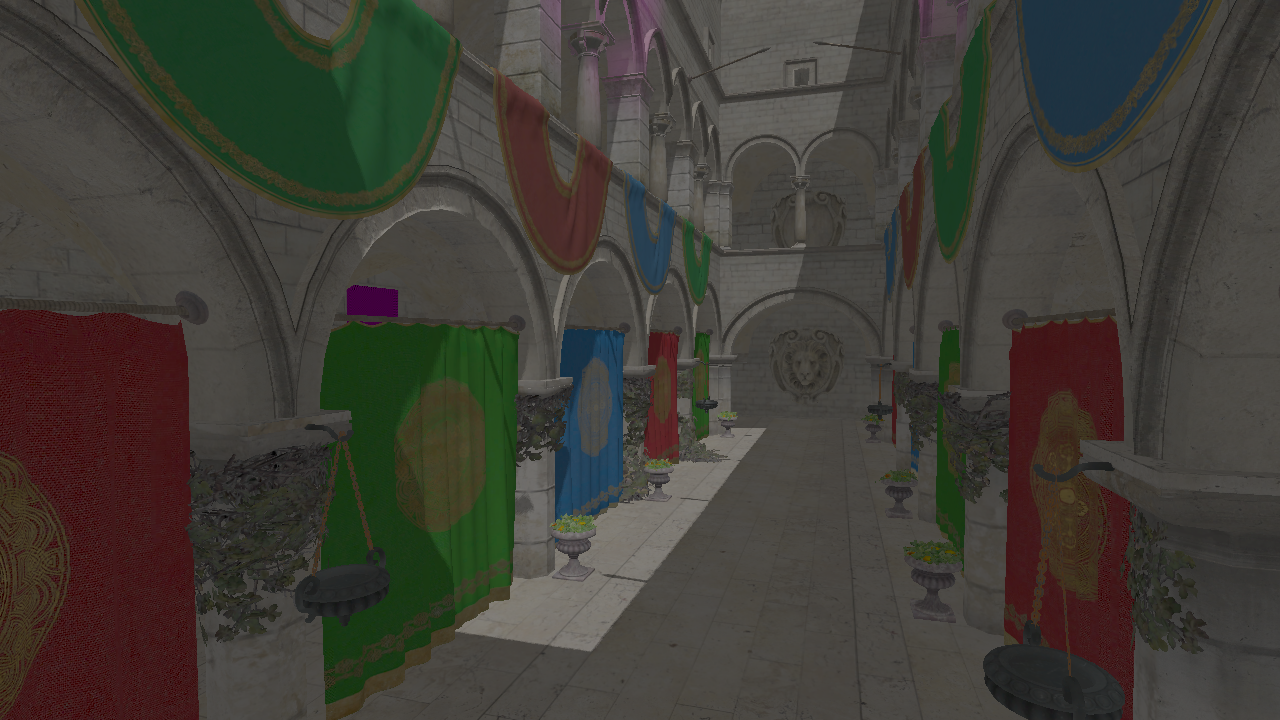
\includegraphics[width=\textwidth]{gi_off.png}
    \caption*{:(}
  \end{figure}
\end{frame}

% to something like _this_, with goodies like glossy reflection, color bleeding, and ambient occlusion
% These effects are from approximating the indirect light in the scene: the light that doesn't come directly from a light source.
\begin{frame}{Motivations}
  \begin{figure}
    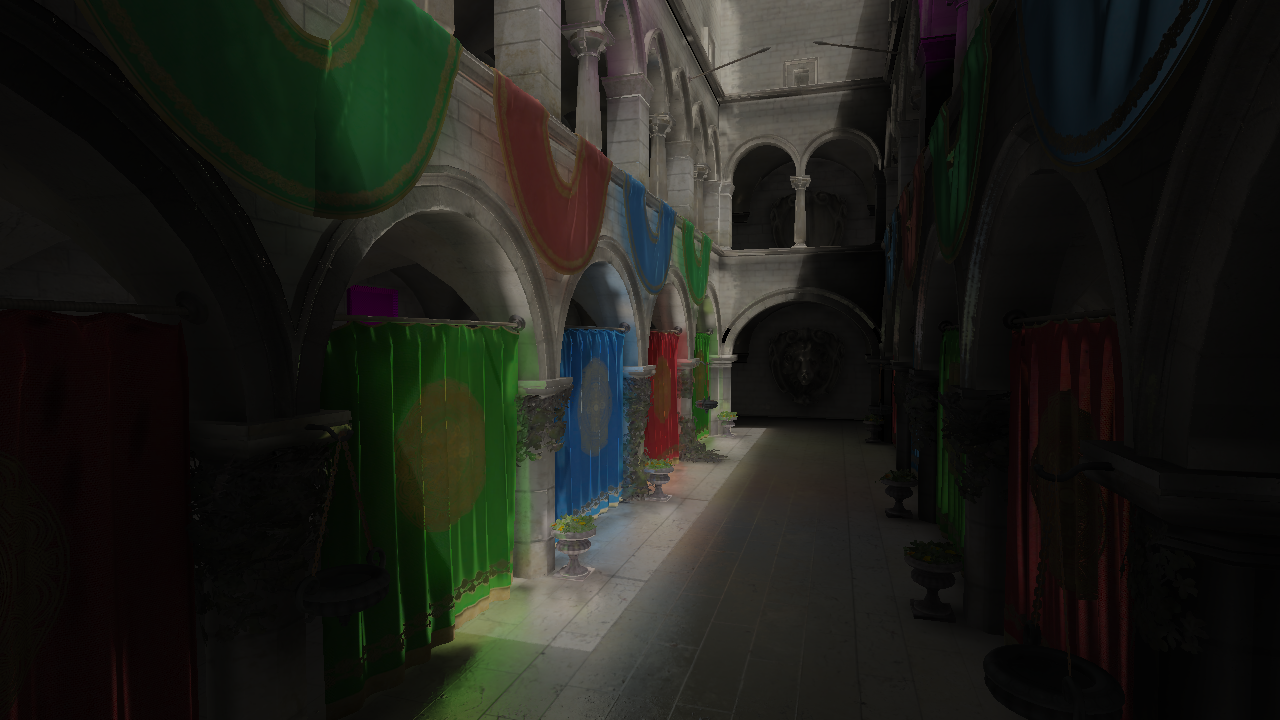
\includegraphics[width=\textwidth]{gi_on.png}
    \caption*{:)}
  \end{figure}
\end{frame}

% \begin{frame}{Teaser}
% % video or screenshots, show good lighting + moving objects
% \movie[autostart,showcontrols]{\textcolor{black}{\rule{\textwidth}{0.9\textheight}}}{test.webm}
% \end{frame}

% \begin{frame}{What did I just see?}
% % real time gi of course!
% \end{frame}

\subsection{Motivations}
\begin{frame}{Motivations}
  \begin{enumerate}
    % \centering
    \item Real-time global illumination is difficult % lots of computation, most algorithms require a lot of parts so it's difficult to start from scratch (like most of us)
      % \begin{itemize}
      %   \item Approximations need to be as fast and accurate as possible
      %   \item Many steps and stuff to keep track of
      % \end{itemize}
    \item Limited reference material
        % \begin{itemize}
        %   \item Not much public code  % solutions developed in the industry or by researchers often aren't open source (e.g. vxgi is binary, code accompanying research papers not there or perhaps integrated into proprietary codebase)
        %   \item Demo or engine code % most is limited in scope or is tied to an engine, making it difficult to extend or integrate into your own project
        % \end{itemize}
    % \pause
    % \item It's cool % the real reason tbh
  \end{enumerate}
\end{frame}

\subsection{Contributions}
\begin{frame}{Contributions}
  \begin{itemize}
    \item Open-source, cross-platform implementation of real-time global illumination % except for apple since they don't like opengl. the big goal here is for others to be able to work on it and do cool stuff (jaafer already used the vct part :) ). voxel cone tracing is the general technique used to achieve gi
    \item Comparison of two different methods of scene voxelization % voxelization is an important part of many new gi algorithms so we wanted to compare two different methods
    \item Investigation into warped (nonuniform size) voxels % more on this later, first I'd like to give a crash course in graphics and an overview of other solutions to real time gi
  \end{itemize}
\end{frame}

\section{Background}

% Please stop me and ask for clarification or more info!

\subsection{Computer Graphics}
\begin{frame}{Computer Graphics Primer}
  \begin{block}{Goal}
    Given a virtual description of a scene, render an image.
  \end{block}

  \begin{block}{Big Issues}
    \begin{enumerate}
      \item How do we represent a scene? What information is required?  % geometry (triangles, voxels), materials (colors, properties), lights (type, position, color, direction), etc.
      \item How is a 3D scene represented as a 2D image?  % implies some transformation needed. we'll also quickly look at how the GPU accomplishes this since it'll help when explaining stuff later
      \item How do we render---how is the final pixel color computed? % lighting/shading model; this is the focus of this thesis
    \end{enumerate}
  \end{block}
  % rtr objects -> world space -> screen space
  % goal of computer graphics; graphics pipeline; transforms and other common stuff
\end{frame}

\begin{frame}{How do we represent a scene?}
  % \setbeamercovered{transparent}
  \begin{columns}
    \begin{column}{0.5\textwidth}
      \begin{description}[<+>]
        \item[Geometry] triangles, voxels % triangles inherently 2D->good for surfaces, not so much for volumetric data. recent gpu developments have made working with nontriangle data more viable, which is why the voxel representation is gaining popularity
        \item[Materials] colors and other properties % albedo + roughness, normal maps (kinda)
        \item[Lights] positions, colors, etc.
      \end{description}
    \end{column}
    \begin{column}{0.5\textwidth}
      \only<1>{
        \begin{figure}
          \begin{subfigure}{\textwidth}
            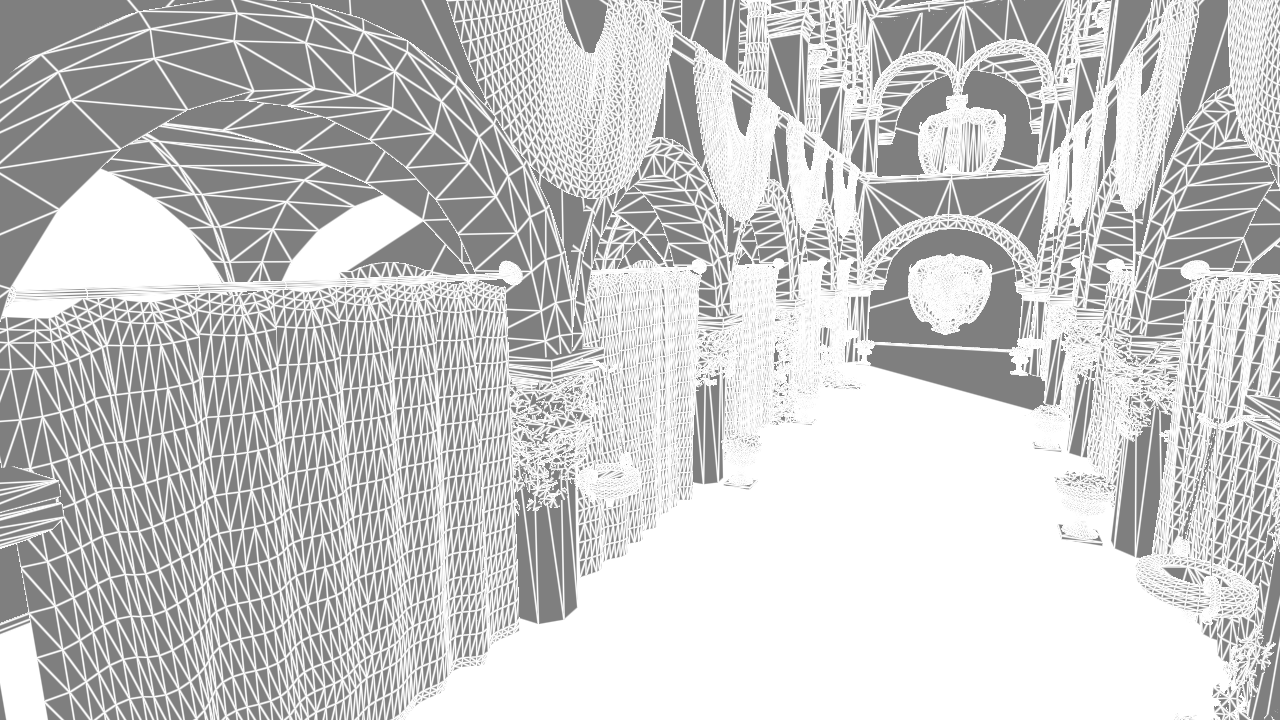
\includegraphics[width=\textwidth]{wireframe.png}
          \end{subfigure}
          \begin{subfigure}{\textwidth}
            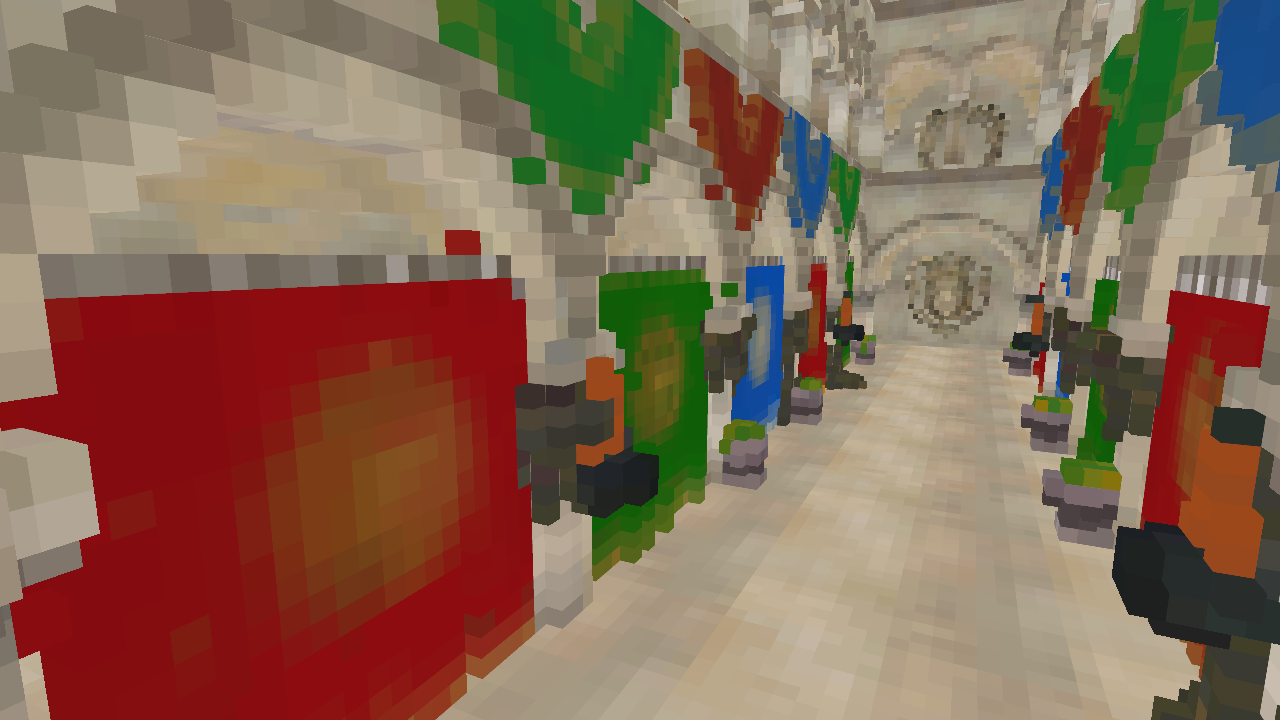
\includegraphics[width=\textwidth]{voxels.png}
          \end{subfigure}
        \end{figure}}

      \only<2>{
        \begin{figure}
          \begin{subfigure}{\textwidth}
            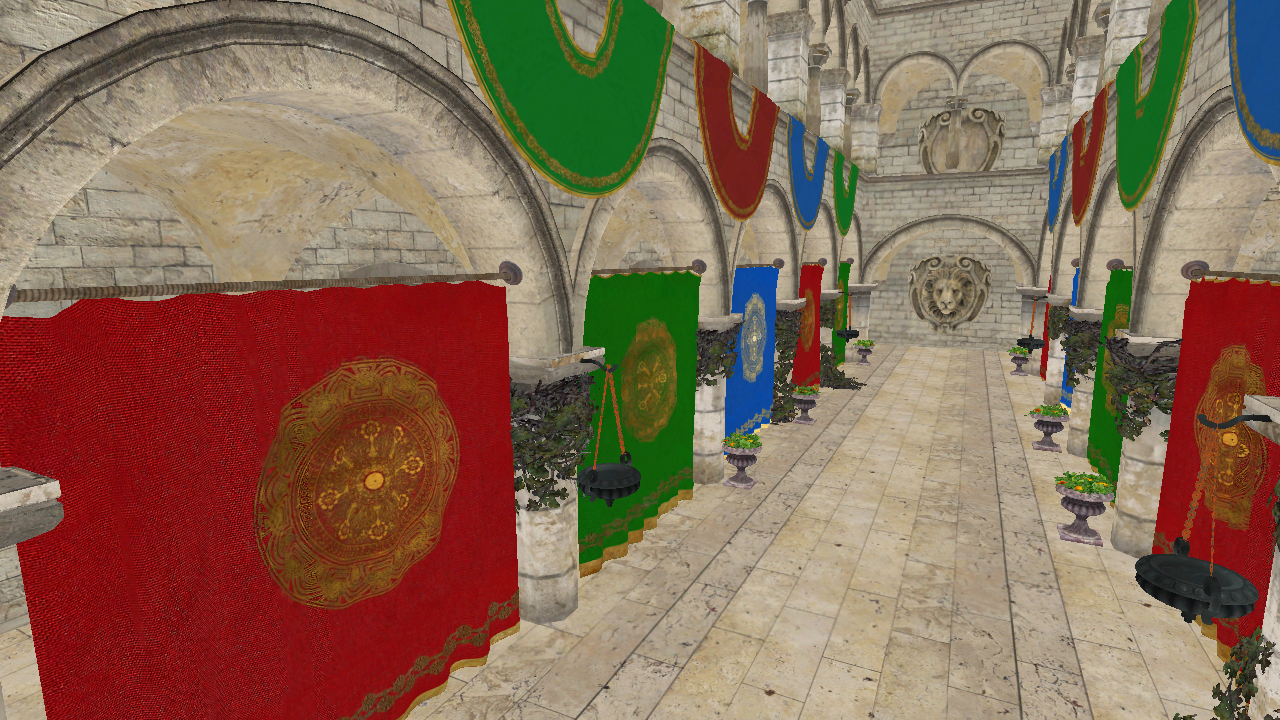
\includegraphics[width=\textwidth]{albedo.png}
          \end{subfigure}
          \begin{subfigure}{\textwidth}
            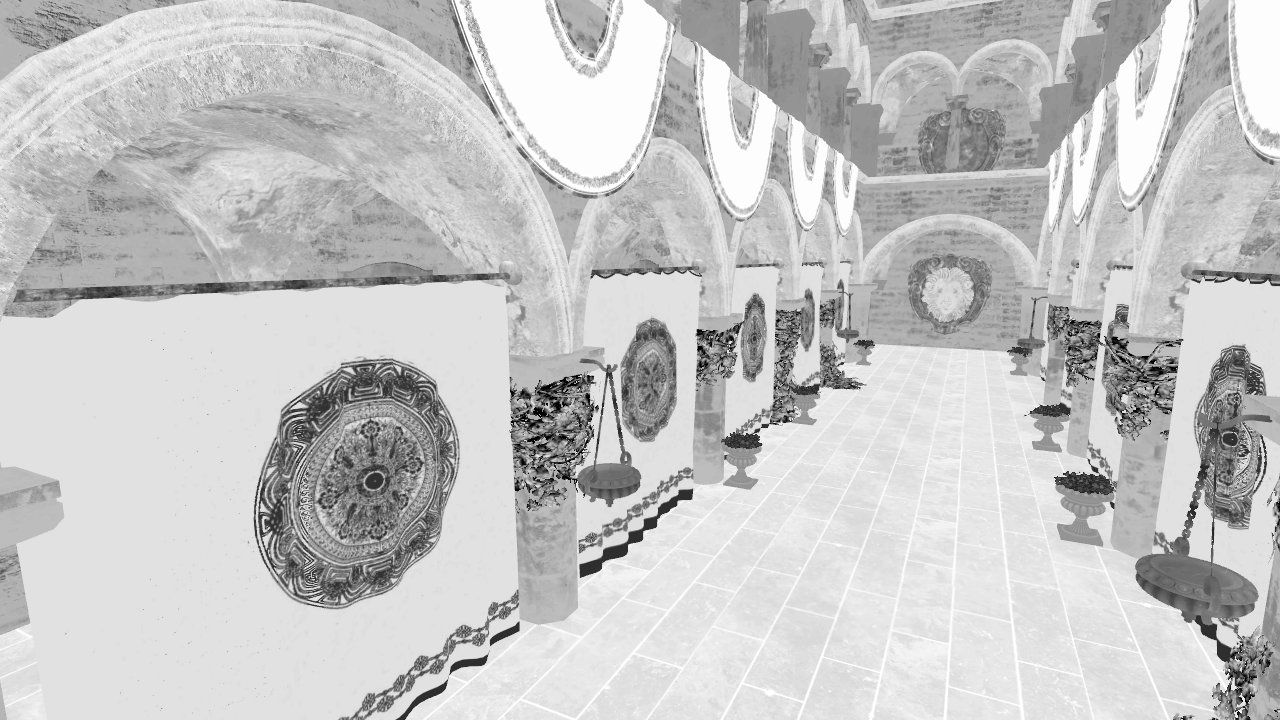
\includegraphics[width=\textwidth]{roughness.png}
          \end{subfigure}
        \end{figure}}

      \only<3>{
        \begin{figure}
          \begin{subfigure}{\textwidth}
            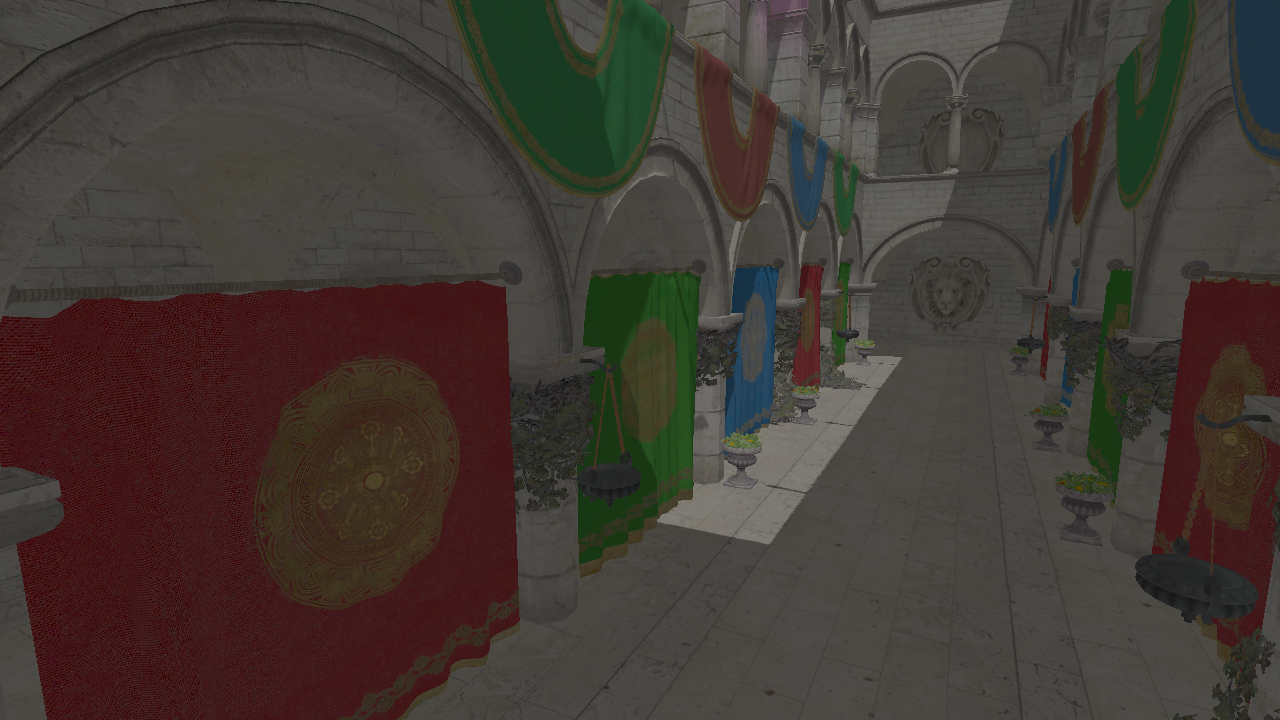
\includegraphics[width=\textwidth]{nogi.png}
          \end{subfigure}
          \begin{subfigure}{\textwidth}
            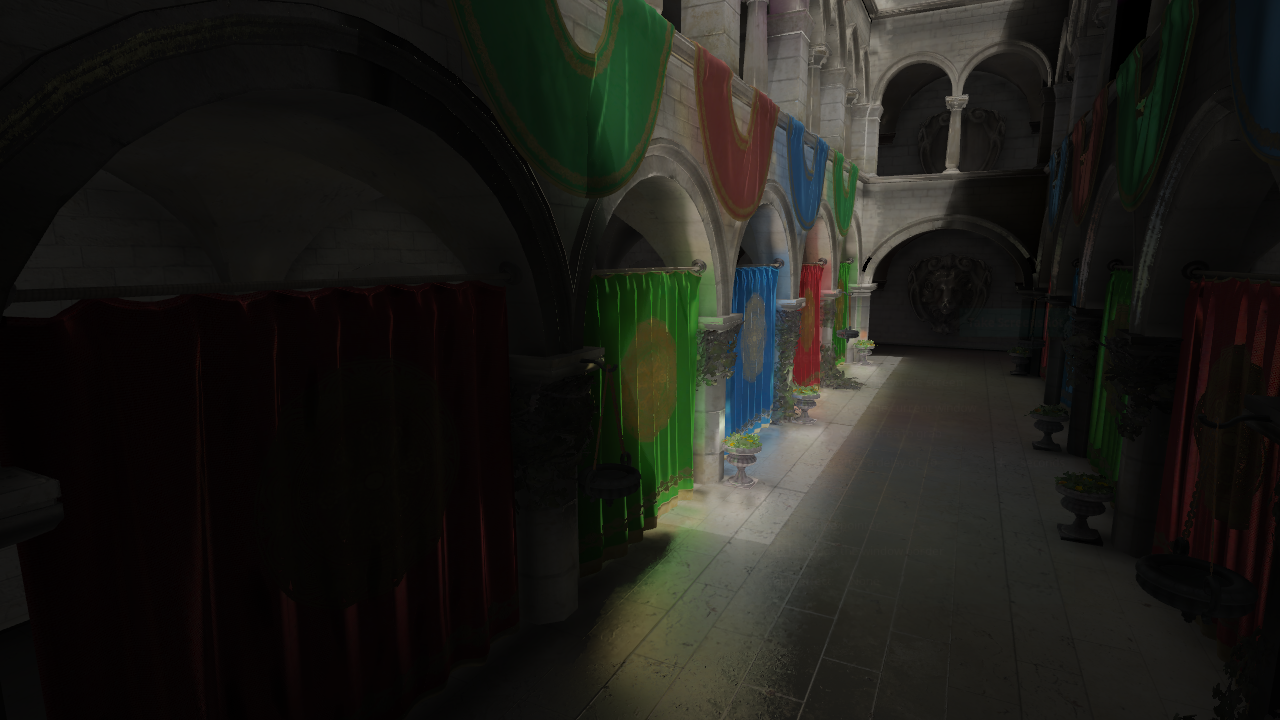
\includegraphics[width=\textwidth]{gi.png}
          \end{subfigure}
        \end{figure}}
    \end{column}
  \end{columns}
\end{frame}

% The second question was how to represent 3D objects in 2D. Once the objects are defined in a common coordinate system, we define this view frustum which determines the objects we'll see. From there we can apply a projection to get a 2D position along with a depth.
{\setbeamertemplate{frame footer}{image from Real-Time Rendering} % TODO cite
\begin{frame}{How is a 3D scene represented as a 2D image?}
  Math!

  All coordinates are transformed multiple times before ending up at their appropriate place on the screen.

  \begin{figure}
    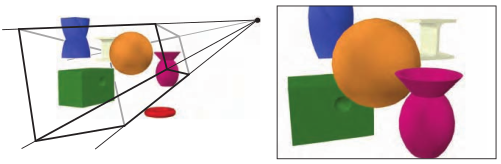
\includegraphics[width=\textwidth]{rtr_fig2_1.png}
  \end{figure}

\end{frame}}

% % The typical transformation to transform any vertex from a typical triangle mesh to its final spot on the screen is shown here. The important step here is getting the vertices into view space, which Keeping track of which space you're working in for lighting and other computations is super important.
% \begin{frame}{How is a 3D scene represented as a 2D image?}
%   % picture of coordinate systems and give brief explanation, since explain more along with the graphics pipeline
%   % showing this so everyone is comfortable when explaining algorithms
%   % ...and this is accomplished with <flick> THE GRAPHICS PIPELIIIIIIINE

%   \begin{figure}
%     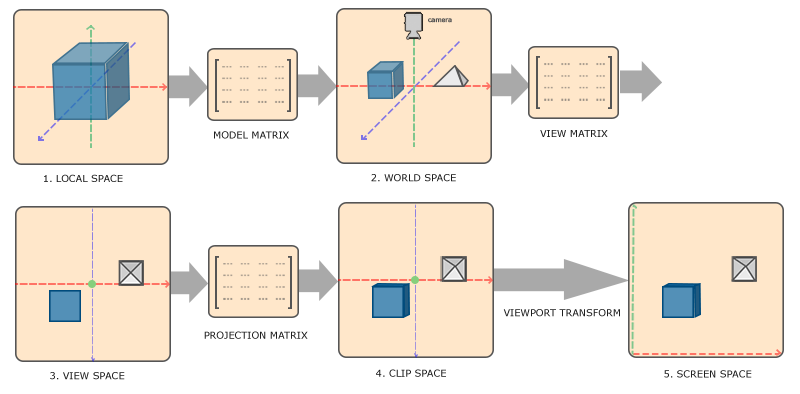
\includegraphics[width=\textwidth]{learnopengl_coordinate_systems.png}
%   \end{figure}

%   % \begin{description}[<+| only@+>]
%   %   \item[Local/Object Space] coordinate system relative to a single object
%   %   \item[World Space] a global coordinate system for the virtual world
%   %   \item[View Space] coordinates are with respect to the camera
%   %   \item[Clip Space/NDC] defines a frustum in which objects will be rasterized % those outside the frustum are clipped
%   %   \item[Screen Space] coordinates are the pixel position and a depth value
%   % \end{description}

%   % Also other spaces, like texture space [0, 1], image space (integral coordinates),

% \end{frame}

{\setbeamertemplate{frame footer}{\href{https://learnopengl.com/img/getting-started/pipeline.png}{image} by \href{https://twitter.com/JoeyDeVriez}{Joey de Vries}, \href{https://creativecommons.org/licenses/by/4.0/}{CC BY 4.0}}
\begin{frame}{How is a 3D scene represented as a 2D image?}
  \begin{center}
    \huge\textbf{The Graphics Pipeline}
  \end{center}
  % This is the standard sequence of events that render the final image from our scene. For nonstandard stuff like voxelization these stages are often abused to increase performance.
  % We'll go over the entire pipeline for sake of completess
  \begin{figure}
    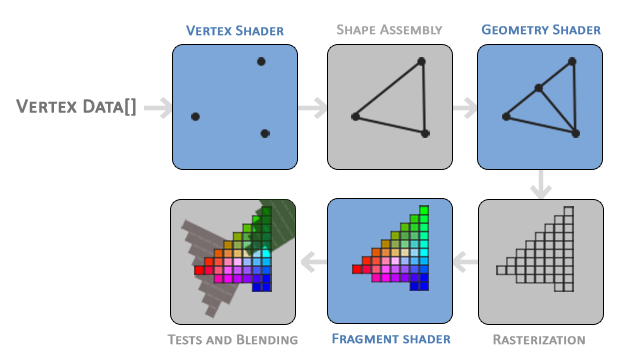
\includegraphics[width=\textwidth]{learnopengl_graphicspipeline.png}
  \end{figure}
\end{frame}}

% \begin{frame}{The Graphics Pipeline}
%   \begin{figure}
%     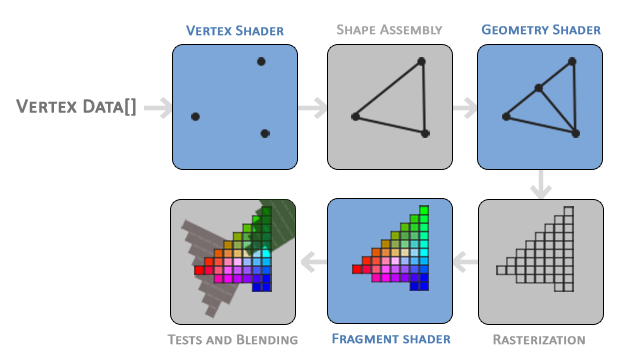
\includegraphics[width=\textwidth]{learnopengl_graphicspipeline.png}
%   \end{figure}

%   \begin{description}[<+| only@+>]
%     \item[Input] A series of vertices containing attributes like position, normal, and texture coordinates.
%     \item[Vertex Shading] Executed for each vertex. Usually applies transforms.
%     \item[Shape Assembly] Form geometric primitives from vertices (like triangles). Tessellation, a way to subdivide points, can also occur around here.
%     \item[Geometry Shading] Operate on primitives.
%     \item[Rasterization] Generate fragments for pixels covered by primitives.
%     \item[Fragment Shading] Executed for each fragment. Usually shading occurs here.
%     \item[Testing and Blending] Depth testing and alpha blending.
%   \end{description}

%   % There are also compute shaders for operating on arbitrary data and tessellation shaders for dynamically subdividing primitives (as we'll see in a bit).
% \end{frame}

% \begin{frame}{Compute Shader}
%   % just want to introduce the concept since I'll mention them in implementation
% \end{frame}

% \begin{frame}{Tessellation}
%   % briefly go over triangle tessellation and where it fits in the pipeline. will probably talk about it more in implementation

%   \begin{figure}
%     
\includegraphics[height=\textheight]{openglwiki_tesselation.png}
%   \end{figure}
% \end{frame}

\subsection{Lighting}
{\setbeamertemplate{frame footer}{\href{http://on-demand.gputechconf.com/gtc/2012/presentations/SB134-Voxel-Cone-Tracing-Octree-Real-Time-Illumination.pdf}{image from VCT and SVO for Real-time Global Illumination} by Cyril Crassin}
\begin{frame}{How do we render?}
  % We need a shading model: a way to compute a color from the geometry, lights, and materials we have in the scene for a particular point
  % Makes sense to model this based on the real-world sooo
  \begin{figure}
    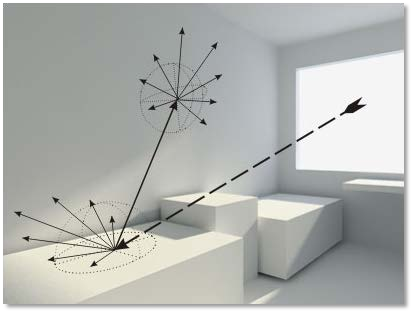
\includegraphics[height=0.9\textheight]{indirectlighting}
  \end{figure}
\end{frame}}

\begin{frame}{Light Theory}
  % Lighting algorithms are numerical approximations
  % The direct light is relatively straightforward to compute: for each point we can iterate through all the lights and sum their contributions
  % Indirect light is the hard part, since the light can come from anywhere in the scene. To figure out all the light in the scene we'd have to test every possible direction in this hemisphere. Therefore we have to resort to approximations...
  % Often the spots where indirect light comes from like right here on the wall are called virtual point lights. The idea is that they behave like normal light sources but they're virtual because the light is essentially sourced from somewhere else (the primary light sources)

  \begin{figure}
    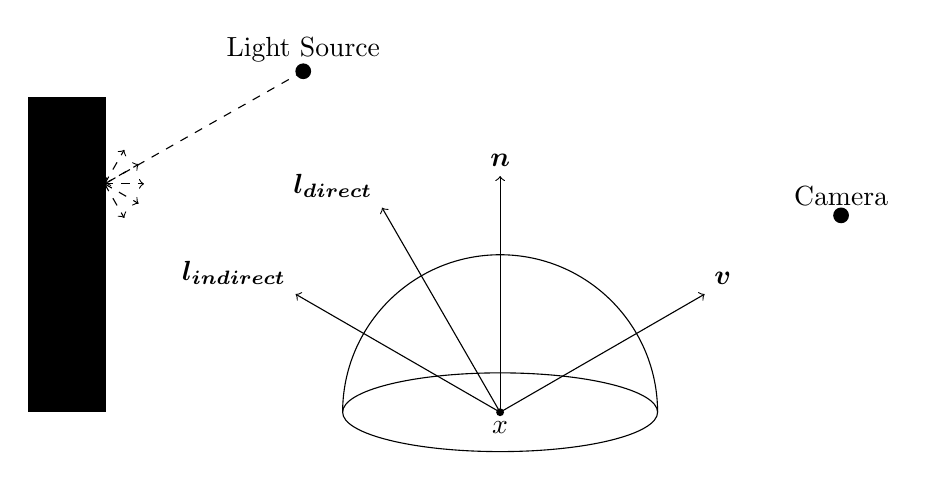
\begin{tikzpicture}
      \draw (2, 0) arc (0:180:2);
      \draw (0, 0) ellipse (2cm and 0.5cm);

      \fill (0, 0) circle (0.05cm) node[below] (x) {$x$};

      \draw[->] (0, 0) -- (30:3cm) node[above right] {$\bm{v}$};
      \draw[->] (0, 0) -- (90:3cm) node[above] {$\bm{n}$};
      \draw[->] (0, 0) -- (120:3cm) node[above left] {$\bm{l_{direct}}$};
      \draw[->] (0, 0) -- (150:3cm) node[above left] {$\bm{l_{indirect}}$};

      \path (30:5cm) coordinate (camera);
      \fill (camera) circle (0.1cm) node[above] {Camera};

      \path (120:5cm) coordinate (light);
      \fill (light) circle (0.1cm) node[above] {Light Source};

      \path (150:5.8) coordinate (bounce);
      \fill (-6, 0) rectangle (-5, 4);
      \path (bounce) circle (0.1cm);
      \draw[dashed, ->] (light) -- (bounce);
      \foreach \angle in {60, 30, 0, -30, -60} {
        \draw[dashed, ->] (bounce) -- +(\angle:0.5cm);
      }
    \end{tikzpicture}
  \end{figure}

  % TODO rendering equation?
\end{frame}

% There are many different ways to achieve global illumination, often with very different goals and tradeoffs. Also, most complete lighting solutions combine multiple independent techniques or only selectively apply them in order to meet quality, time, and memory constraints.
% The first approach to computing indirect light is essentially to not compute it and just use a constant factor. This is of course very fast but not accurate at all.
% Next we have 'partial' global illumination approaches. While better, these methods don't attempt to fully simulate indirect lighting---they're hacks.
% Static methods involve precomputing lighting prior to runtime. The lighting quality itself is often very accurate, but it doesn't handle dynamic, moving objects.
% Lastly, we have the dynamic approaches. The entire algorithm is designed to fit inside a single frame so all dynamic objects have their light updated (of course there are tricks and speed this up). This is what we are interested in.
\begin{frame}{Real-Time Global Illumination}
  Various approaches to approximating indirect light.

  \begin{description}
    \item[Constant] Fixed fraction of ambient light % as seen in first image
    \item[Partial] Ambient occlusion, screen space reflections % only model parts of global illumination; often local methods that do not have complete scene information
    \item[Static] Baked lighting, light probes
    \item[Dynamic] Reflective Shadowmaps, Light Propagation Volumes, Voxel Cone Tracing
  \end{description}
\end{frame}

% Most algorithms end up having the same main steps. The differences generally come from what the representation is (volumetric? screen space? is it complete or just local?) and how it's stored (if any special data structure is used). When doing the final gathering of the light there's often a clever way to sample the lighting to reduce computations.
\begin{frame}{Real-Time Global Illumination}
  Most dynamic global illumination algorithms follow a few main steps:

  \begin{enumerate}
    \item Construct representation of the scene
    \item Calculate indirect lighting information
    \item Collect indirect lighting when rendering
  \end{enumerate}

  % So for our algorithm the first thing we do is voxelize the scene so we have a volumetric representation. Then, we place our indirect light sources (vpls) into the voxels and downsample it. Finally, we use voxel cone tracing to sample the indirect light from the voxels.
\end{frame}

% \begin{frame}{Spatial Data Structures}
%   % quickly go through one slide each (with picture)
%   \begin{description}
%     \item<1>[Uniform Texture] each cell is the same size  % simple, hw filtering; wasteful
%     \item<2>[Cascaded Texture/Clipmap] nested textures with varying cell sizes % there is difference but not important for us; cell sizes are discrete multiplies, still wasteful but better, need to handle edges properly
%     \item<3>[Octree] adaptive tree structure which holds values in leaves % sparse, difficult on gpu to build and traverse, no hw filtering
%   \end{description}

%   \begin{figure}
%     % TODO TODO TODO \includegraphics<+>[width=\textwidth]{}
%     \only<1>{\begin{tikzpicture}[scale=0.8]
%       \draw [black, step=1.0] (-4, -4) grid ++(8, 8);
%     \end{tikzpicture}}
%     % \includegraphics<+>[width=\textwidth]{geometry_clipmap.jpg}
%     \only<2>{\begin{tikzpicture}[scale=0.8]
%       \draw [black, step=1.0] (-4, -4) grid ++(8, 8);
%       \draw [black, step=0.5] (-2, -2) grid ++(4, 4);
%       \draw [black, step=0.25] (-1, -1) grid ++(2, 2);
%     \end{tikzpicture}}
%     % \includegraphics<3>[width=\textwidth]{octree.png}
%     \only<3>{\begin{tikzpicture}[scale=0.8]
%       \draw [black, step=4.0] (-4, -4) grid ++(8, 8);
%       \draw [black, step=2.0] (0, 0) grid ++(4, 4);
%       \draw [black, step=1.0] (2, 2) grid ++(2, 2);
%       \draw [black, step=1.0] (2, 0) grid ++(2, 2);
%       \draw [black, step=0.5] (2, 1) grid ++(1, 2);
%       \draw [black, step=0.25] (2, 1.5) grid ++(1, 1);
%     \end{tikzpicture}}
%   \end{figure}
% \end{frame}

% raytracing and raymarching? maybe one slide

% ask for any questions or clarification here? (after related work too maybe?)

% \section{Related Work}

% \subsection{VPLs and RSMs}
% \begin{frame}{VPLs and RSMs}
%   % Just want to introduce the concept of VPLs and RSMs are simple way of doing that
%   \begin{description}
%     \item[Virtual Point Lights] Treat arbitrary objects or locations as light sources
%     \item[Reflective Shadow Maps] Treat each pixel of a shadowmap as a VPL % when rendering project point into shadowmap and gather lighting contributions from VPLs; problem is poor occlusion information and only low frequency lighting
%   \end{description}

%   \begin{figure}
%     \includegraphics<+>[width=\textwidth]{rsm.png}
%     \includegraphics<+>[width=\textwidth]{rsm_vpl.png}
%   \end{figure}

%   % another slide for pros/cons?
% \end{frame}

% % LPVs and VCT after implementation? doesn't really help as background info
% \subsection{Light Propagation Volumes}
% \begin{frame}{Light Propagation Volumes}
%   % low frequency but fairly stable, no occlusion (limited info from reusing), cascaded
%   % iterative process to propagate light throughout scene

%   \begin{itemize}
%     \item Store VPLs in a voxel grid
%     \item Iteratively propagate lighting contribution until stable
%   \end{itemize}

%   \begin{figure}
%     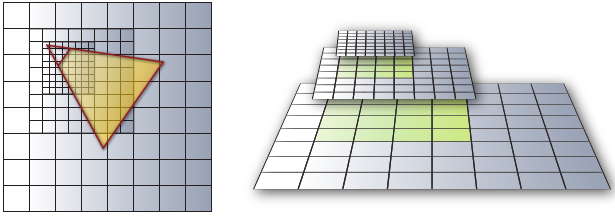
\includegraphics[width=\textwidth]{lpv.png}
%   \end{figure}
% \end{frame}

% \subsection{Voxel Cone Tracing}
% \begin{frame}{Voxel Cone Tracing}
%   % complete occlusion info, sparse voxel octree, specular reflections

%   \begin{itemize}
%     \item Sparse voxel octree % occlusion information
%     \item High resolution (diffuse and specular lighting)
%   \end{itemize}

%   \begin{figure}
%     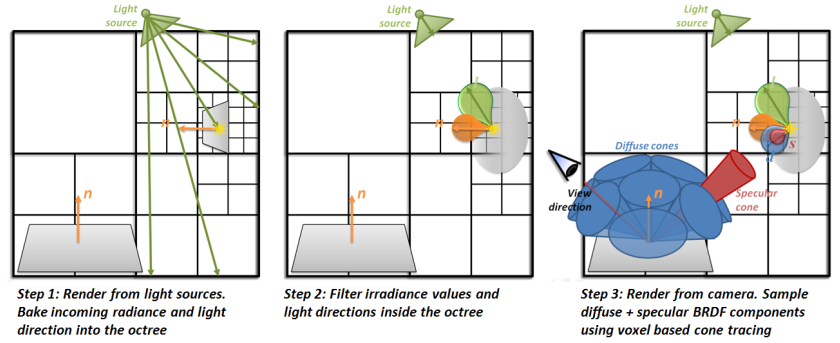
\includegraphics[width=\textwidth]{vct.png}
%   \end{figure}
% \end{frame}

% TODO quick recap here?
% most important bits: voxels represent 3d data well and thus voxelization is important; vpls are core part of most gi algorithms; lpv and vct use regular grid

% \begin{frame}{What am I doing?} % this is the research question
%   % common theme is constructing some (ideally 3D) representation of a scene
%   % we wanted to evaluate an alternate method of voxelization and to see if nonuniform voxel sizes were a promising alternative to existing 3D data structures
%   \begin{enumerate}
%     \item Comparing two approaches for scene voxelization % voxelization is a core part of the algorithm; tessellated version also not restricted to rasterizer
%     \item Investigating continuous voxel sizes % voxel warping; idea is to support bigger scenes and increase resolution near camera without abrupt changes in voxel density
%   \end{enumerate}
% \end{frame}

\section{Implementation}

% \begin{frame}{Overview of Renderer}
%   % flowchart or something showing each render pass
%   % list of all major resources (3ish voxel textures, shadowmap, meshes, materials)

%   % Really what we have is a forward style rendering engine with support for rigid body animation, multiple lights, normal mapping, shadows, and of course global illumination

%   % Step 2 is creating our scene representation
%   % Steps 3, 4, and 5 are computing the indirect lighting information, which we call the radiance texture
%   % Step 6 is where we collect/sample the indirect lighting
%   \begin{columns}
%     \begin{column}{0.5\textwidth}
%       \begin{block}{Main Steps}
%         \begin{enumerate}
%           \item Setup (load scene, create textures, compile shaders)
%           \item Voxelize Scene
%           \item Create Shadowmap
%           \item Inject Radiance
%           \item Filter Radiance
%           % \item Depth Prepass
%           \item Shading
%         \end{enumerate}
%       \end{block}
%     \end{column}
%     \begin{column}{0.5\textwidth}
%       \begin{block}{Important Data}
%         \begin{enumerate}
%           \item Scene (meshes, materials, lights)
%           \item Camera (position, direction) %, projection + view matrices)
%           \item Shadowmap % Framebuffer Object and Texture
%           \item Voxel Textures (color + opacity, normals, radiance)
%         \end{enumerate}
%       \end{block}
%     \end{column}
%   \end{columns}
% \end{frame}

\begin{frame}{Overview of Renderer}
  \captionsetup[subfigure]{font=footnotesize,labelfont=footnotesize}
  \begin{figure}
    \renewcommand{\thesubfigure}{\arabic{subfigure}}
    \begin{subfigure}[t]{0.32\textwidth}
      \adjincludegraphics[width=\textwidth, trim={{0.2\width} {0.1\height} {0.2\width} 0},clip]{gi_step2}
      \caption{Voxelize}
    \end{subfigure}
    \begin{subfigure}[t]{0.32\textwidth}
      \adjincludegraphics[width=\textwidth, trim={{0.2\width} {0.1\height} {0.2\width} 0},clip]{gi_step1}
      \caption{Direct lighting}
    \end{subfigure}
    \begin{subfigure}[t]{0.32\textwidth}
      \adjincludegraphics[width=\textwidth, trim={{0.2\width} {0.1\height} {0.2\width} 0},clip]{gi_step3}
      \caption{Inject direct lighting into voxels}
    \end{subfigure}

    \begin{subfigure}[t]{0.32\textwidth}
      \adjincludegraphics[width=\textwidth, trim={{0.2\width} {0.1\height} {0.2\width} 0},clip]{gi_step4}
      \caption{Filter voxels}
    \end{subfigure}
    \begin{subfigure}[t]{0.32\textwidth}
      \adjincludegraphics[width=\textwidth, trim={{0.2\width} {0.1\height} {0.2\width} 0},clip]{gi_step5}
      \caption{Sample using voxel cone tracing}
    \end{subfigure}
  \end{figure}
\end{frame}

% \AtBeginSubsection[]
% {
% 	\begin{frame}
%       \frametitle{Outline}
%       % \setbeamertemplate{section in toc}[sections numbered]
%         \tableofcontents[currentsection,subsectionstyle=show/shaded/hide]
% 	\end{frame}
% }

\subsection{Voxelization}

{\setbeamertemplate{frame footer}{image from \href{https://www.khronos.org/opengl/wiki/Tessellation}{OpenGL Wiki}}
\begin{frame}{Voxelization with Tessellator}
  \begin{itemize}
    \item Each vertex corresponds to a voxel
    \item Triangles are subdivided into multiple vertices during tessellation
  \end{itemize}

  % Tessellation after vertex shading and before fragment shading
  % rasterizer is not needed (is disabled)

  % Tessellation is a method of programmatically subdividing input primitives (in our case triangles).

  \begin{figure}
    \adjincludegraphics[scale=0.8, trim={0 {0.1\height} 0 0},clip]{openglwiki_tesselation.png}
  \end{figure}
\end{frame}}

\begin{frame}{Determining Tessellation Levels}
  \begin{itemize}
    \item Outer levels determined from respective edge lengths
    \item Inner level determined from maximum triangle altitude length
  \end{itemize}

  % Here is an illustration of the idea behind tessellated voxelization. By subdividing the edges and inside appropriately we can get a fairly good voxelization. A nice part of this voxelization is we don't need to worry about the dominant axis or conservative rasterization.
  \begin{figure}
    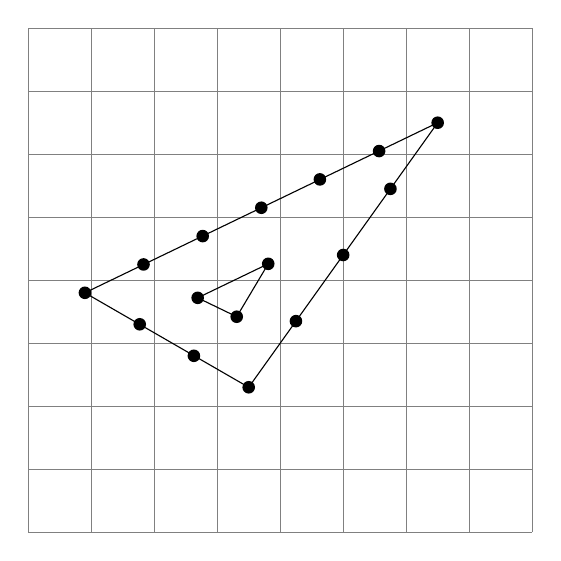
\begin{tikzpicture}[scale=0.8]
      \draw [gray, step=1.0] (-4, -4) grid ++(8, 8);
      \foreach \x/\y in {-3.1/-0.2, -2.23/-0.7, -1.37/-1.2, -0.5/-1.7, 0.25/-0.65, 1.0/0.4, 1.75/1.45, 2.5/2.5, 1.57/2.05, 0.63/1.6, -0.3/1.15, -1.23/0.7, -2.17/0.25, -1.31/-0.28, -0.19/0.26, -0.69/-0.58}{
        \fill[thick, black] (\x, \y) circle (0.1cm);
      }
      \draw [black] (-3.1, -0.2) -- (2.5, 2.5) -- (-0.5, -1.7) -- cycle;
      \draw [black] (-1.31, -0.28) -- (-0.19, 0.26) -- (-0.69, -0.58) -- cycle;
    \end{tikzpicture}
  \end{figure}
\end{frame}

{\setbeamertemplate{frame footer}{image from \href{https://www.seas.upenn.edu/~pcozzi/OpenGLInsights/OpenGLInsights-SparseVoxelization.pdf}{OpenGL Insights: Octree-Based Sparse Voxelization Using the GPU Hardware Rasterizer} by Cyril Crassin and Simon Green}
\begin{frame}{Voxelization with Rasterizer}
  Each fragment corresponds to a voxel
  % since fragments are inherently 2D, we use the depth value to recreate the 3D coordinates. Also, since the rasterization is in 2D, we have to make sure we view the triangle from the direction that'll maximize its 2D area. Once we have the fragment we can figure out its voxel position and write it in. Now for the conservative rasterization...

  \begin{figure}
    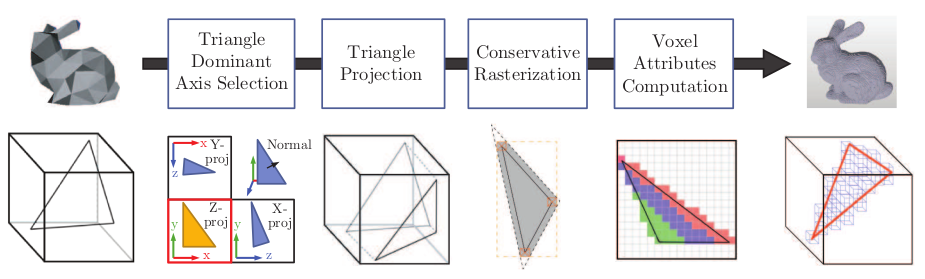
\includegraphics[width=\textwidth]{rasterizedvoxelization}
  \end{figure}
\end{frame}}

{\setbeamertemplate{frame footer}{images by Jon Story from \href{https://developer.nvidia.com/content/dont-be-conservative-conservative-rasterization}{Don't be conservative with Conservative Rasterization}}
\begin{frame}{Conservative Rasterization}
  % Of particular importance with the rasterization approach is the need for conservative rasterization. In general, a fragment is only generated for a triangle if that triangle overlaps the center of the fragment (pixel). This can cause undesirable cracks and holes in the voxelization. Conservative rasterization is meant to address this by generating a fragment for even partially overlapped fragments.

  \begin{figure}
    \begin{subfigure}[t]{0.475\textwidth}
      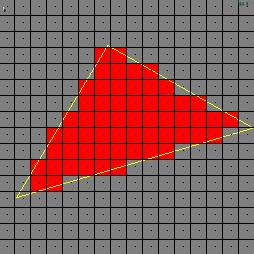
\includegraphics[width=\textwidth]{conservativeraster_off}
      \caption*{Off}
    \end{subfigure}
    ~
    \begin{subfigure}[t]{0.475\textwidth}
      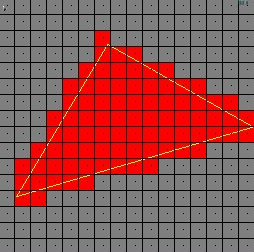
\includegraphics[width=\textwidth]{conservativeraster_on}
      \caption*{On}
    \end{subfigure}
  \end{figure}
\end{frame}}

\begin{frame}{Conservative Rasterization}
  % Here is a comparison between no conservative rasterization and with. We use an MSAA based method (a good compromise between simplicity, quality, and it's cross vendor)

  \begin{figure}
    \begin{subfigure}[t]{0.475\textwidth}
      \adjincludegraphics[width=\textwidth,trim={0 0 {0.5\width} 0},clip]{voxels_off}
      \caption*{Off}
    \end{subfigure}
    ~
    \begin{subfigure}[t]{0.475\textwidth}
      \adjincludegraphics[width=\textwidth,trim={0 0 {0.5\width} 0},clip]{voxels_msaa}
      \caption*{On}
    \end{subfigure}
  \end{figure}
\end{frame}

\subsection{Radiance Injection and Filtering}
% \begin{frame}{Radiance Injection}
%   \begin{itemize}
%     \item Create virtual point lights for all geometry hit by the light.
%     \item These lights approximate a single-bounce of indirect lighting.
%   \end{itemize}

%   \begin{figure}
%     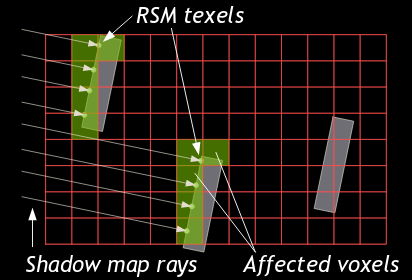
\includegraphics[width=0.8\textwidth]{lightinjection}
%   \end{figure}
% \end{frame}

{\setbeamertemplate{frame footer}{left image from \href{http://on-demand.gputechconf.com/gtc/2014/presentations/S4552-rt-voxel-based-global-illumination-gpus.pdf}{Practical Real-time Voxel-based Global Illumination for Current GPUs} by Alexey Panteleev}
\begin{frame}{Radiance Injection}
  Use \textbf{shadowmap} to determine where direct light hits voxels

  % Only interested in depth values important for us: along with the light matrix we can reconstruct world positions
  % picture
  % implementation? ortho matrix, projection

  % \begin{figure}
  %   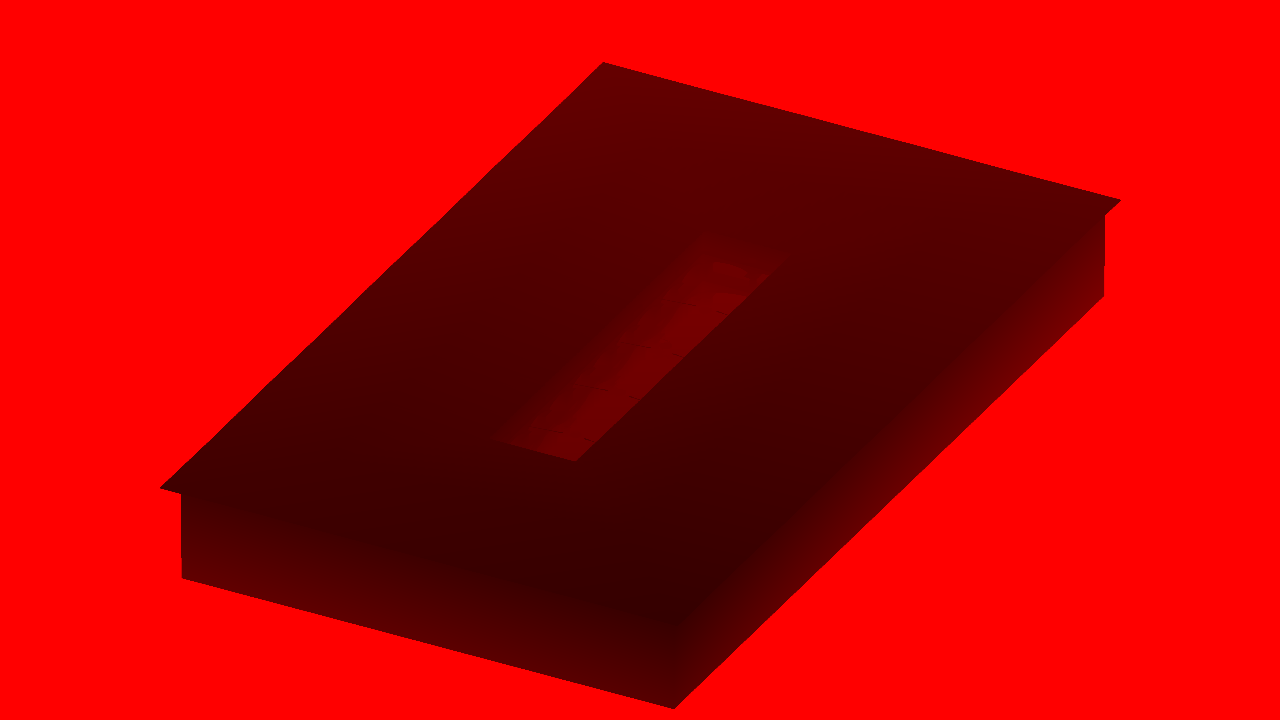
\includegraphics[width=0.8\textwidth]{shadowmap}
  % \end{figure}
  \begin{figure}
    % \begin{subfigure}[t]{0.475\textwidth}
    %   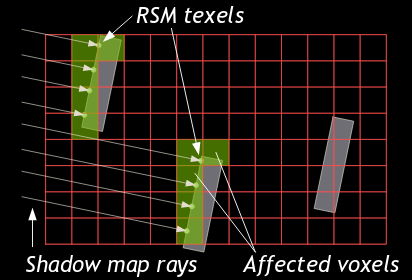
\includegraphics[width=\textwidth]{lightinjection}
    % \end{subfigure}
    % ~
    % \begin{subfigure}[t]{0.475\textwidth}
      \adjincludegraphics[width=0.8\textwidth,trim={{0.1\width} 0 {0.1\width} 0},clip]{shadowmap}
    % \end{subfigure}
  \end{figure}
\end{frame}}

{\setbeamertemplate{frame footer}{left image from \href{http://on-demand.gputechconf.com/gtc/2014/presentations/S4552-rt-voxel-based-global-illumination-gpus.pdf}{Practical Real-time Voxel-based Global Illumination for Current GPUs} by Alexey Panteleev}
\begin{frame}{Radiance Injection}
  Use \textbf{shadowmap} to determine where direct light hits voxels

  \begin{figure}
    \begin{subfigure}[t]{0.475\textwidth}
      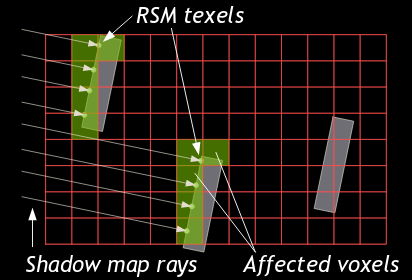
\includegraphics[width=\textwidth]{lightinjection}
    \end{subfigure}
    ~
    \begin{subfigure}[t]{0.475\textwidth}
      \adjincludegraphics[width=\textwidth,trim={0 0 {0.2\width} 0},clip]{radiance_nolighting}
    \end{subfigure}
  \end{figure}
\end{frame}}

% Now that we have a high resolution version of the light in the scene we want to smooth it out. This step is for mimicing how light should spread out and bounce around. The number of levels (the mipmaps) of filtered light is a configurable parameter and each level is half the size of the previous. To compute the next level we just average neighboring voxels.
\begin{frame}{Radiance Filtering}
  \begin{itemize}
    \item Multiple \textbf{levels} (mipmaps)
    \item Each level is half the size of the previous
    \item Computing the next level is a 2x2x2 average
  \end{itemize}

  \begin{center}
    \definecolor{purple}{rgb}{1.0, 0.0, 1.0}
    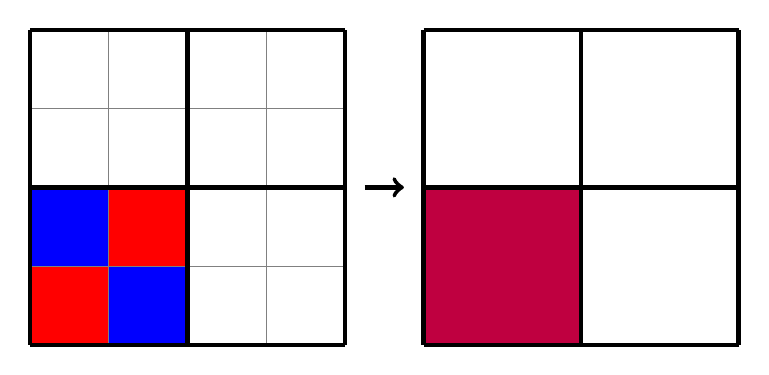
\begin{tikzpicture}
      \fill[red] (0, 0) rectangle (1, 1);
      \fill[red] (1, 1) rectangle (2, 2);
      \fill[blue] (1, 0) rectangle (2, 1);
      \fill[blue] (0, 1) rectangle (1, 2);
      \fill[{purple}] (5, 0) rectangle (7, 2);

      \draw[step=1.0, gray] (0, 0) grid (4, 4);
      \draw[step=2.0, black, ultra thick] (0, 0) grid (4, 4);
      \draw[black, ->, ultra thick] (4.25, 2) to (4.75, 2);
      \draw[step=2.0, black, ultra thick, xshift=5.0cm] (0, 0) grid (4, 4);
    \end{tikzpicture}
  \end{center}
\end{frame}

% the cracks are the result of imperfect voxelization (conservative rasterization)
% also this is only showing the surface values, the empty space also contains semi-opaque colors
\begin{frame}{Radiance Filtering}
  % \begin{figure}
  %   \includegraphics<+>[width=\textwidth]{mipmap0.png}
  %   \includegraphics<+>[width=\textwidth]{mipmap1.png}
  %   \includegraphics<+>[width=\textwidth]{mipmap2.png}
  %   \includegraphics<+>[width=\textwidth]{mipmap3.png}
  %   \caption*{\only<1>{Mipmap level 0}\only<2>{Mipmap level 1}\only<3>{Mipmap level 2}\only<4>{\\Mipmap level 3}}
  % \end{figure}
  \begin{figure}
    \centering
    \begin{subfigure}[b]{0.475\textwidth}
        \centering
        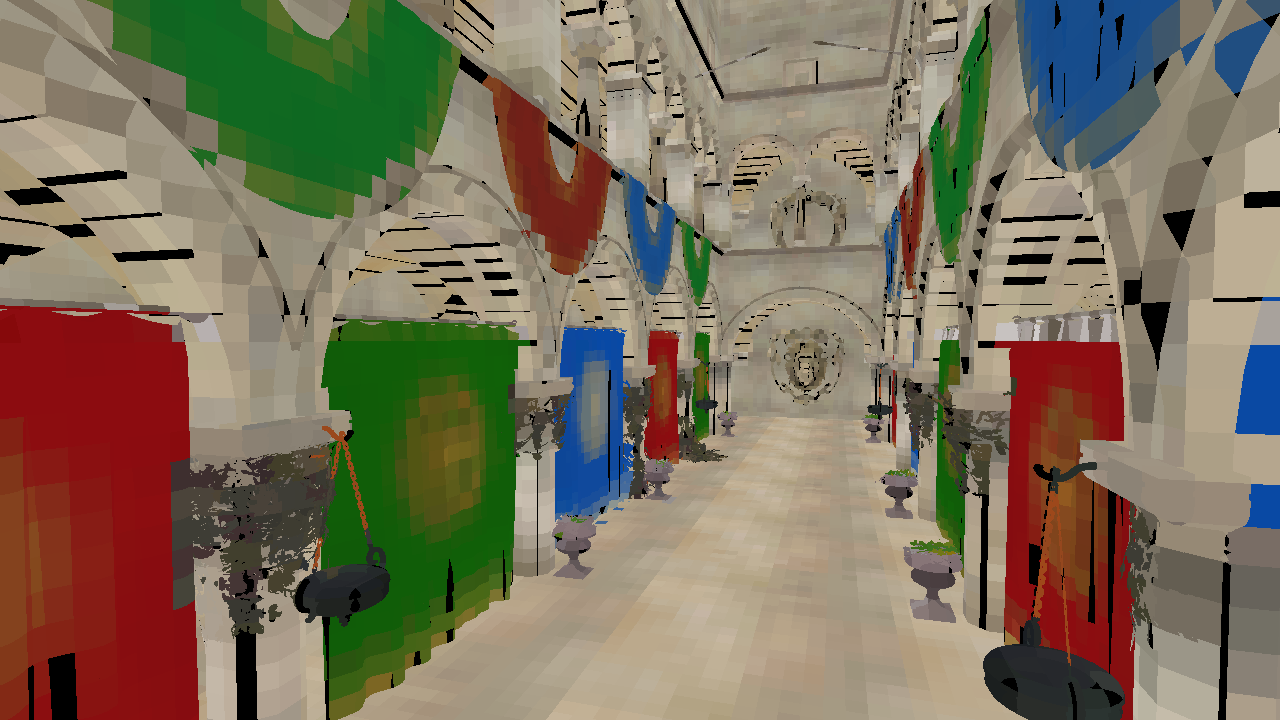
\includegraphics[width=\textwidth]{mipmap0.png}
        \caption*{Level 0}
    \end{subfigure}
    \hfill
    \begin{subfigure}[b]{0.475\textwidth}
        \centering
        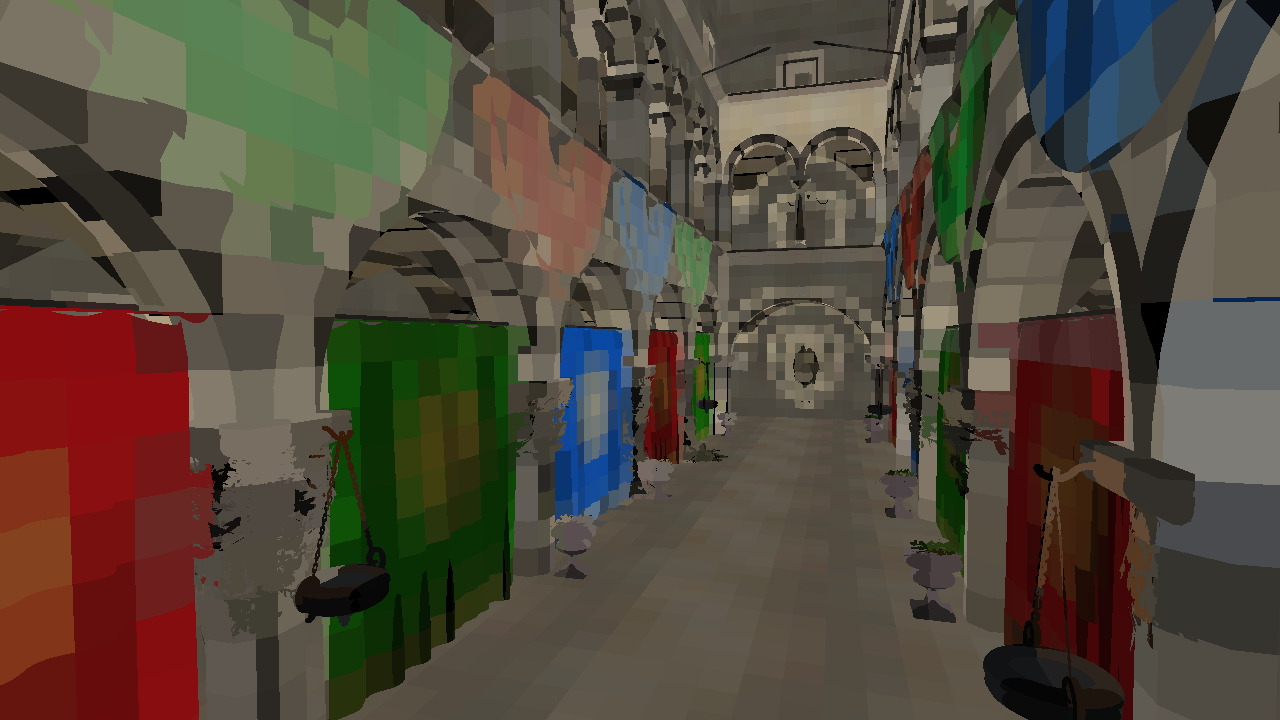
\includegraphics[width=\textwidth]{mipmap1.png}
        \caption*{Level 1}
    \end{subfigure}
    % \vskip\baselineskip

    \begin{subfigure}[b]{0.475\textwidth}
        \centering
        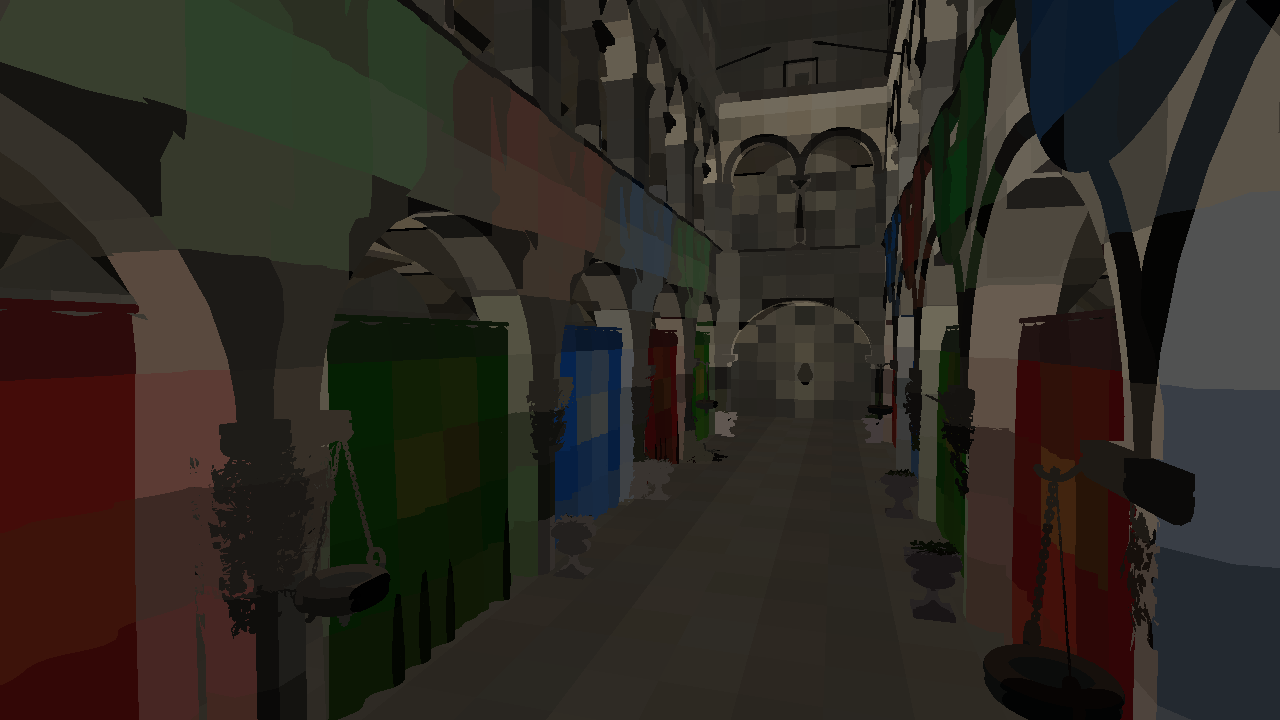
\includegraphics[width=\textwidth]{mipmap2.png}
        \caption*{Level 2}
    \end{subfigure}
    \quad
    \begin{subfigure}[b]{0.475\textwidth}
        \centering
        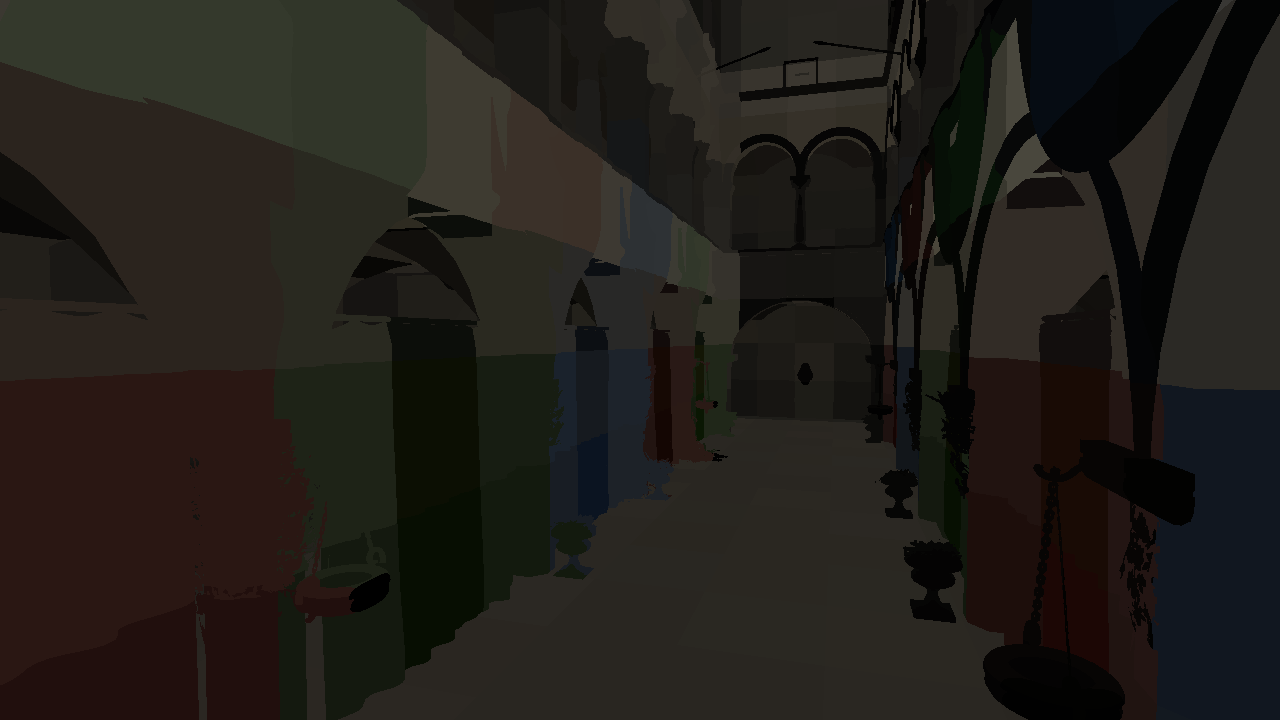
\includegraphics[width=\textwidth]{mipmap3.png}
        \caption*{Level 3}
    \end{subfigure}
    \caption*{Mipmaps}
  \end{figure}
\end{frame}

\subsection{Final Shading}

% TODO remove?
% \begin{frame}{Depth Prepass}
%   \begin{itemize}
%     \item Shading (on each pixel) is expensive
%     \item Use the depth buffer to ensure only the final pixels are shaded
%   \end{itemize}

%   %An optimization to minimize the number of shaded fragments.

%   %Prefill the depth buffer so lighting (including the relatively expensive voxel cone tracing) will only be performed on the visible fragments of the scene. % remind of depth test and this is only for forward rendering (deferred already does this when creating gbuffer)
% \end{frame}

% \begin{frame}{Final Shading}
%   \begin{description}
%     \item[Direct Lighting] Cook-Torrance shading model
%     \item[Indirect Lighting] voxel cone tracing
%     \item[Post Processing] tone mapping and gamma correction
%   \end{description}
% \end{frame}

% Computing the direct lighting is fairly straightforward: we loop through each light and, if the light source isn't being blocked by anything, add the lighting contribution. This computeLighting is based on material properties, light color and intensity, and these vectors: the view vector, surface normal, and light vector.
% \begin{frame}{Direct Lighting}
%   % psuedocode? or just picture of direct light and explain?
%   \begin{algorithm}[H]
%     \begin{algorithmic}
%       \State {color = 0}
%       \For {each light in the scene}
%         \If {not in shadow}
%           \State {color += computeLighting()}
%         \EndIf
%       \EndFor
%     \end{algorithmic}
%   \end{algorithm}

%   \begin{figure}
%     \begin{tikzpicture}[scale=0.7]
%       \draw (2, 0) arc (0:180:2);
%       \draw (0, 0) ellipse (2cm and 0.5cm);

%       \fill (0, 0) circle (0.05cm) node[below] (x) {$x$};

%       \draw[->] (0, 0) -- (30:3cm) node[above right] {$\bm{v}$};
%       \draw[->] (0, 0) -- (90:3cm) node[above] {$\bm{n}$};
%       \draw[->] (0, 0) -- (120:3cm) node[above left] {$\bm{l_{direct}}$};

%       \path (30:5cm) coordinate (camera);
%       \fill (camera) circle (0.1cm) node[above] {Camera};

%       \path (120:5cm) coordinate (light);
%       \fill (light) circle (0.1cm) node[above] {Light Source};
%     \end{tikzpicture}
%   \end{figure}
% \end{frame}

% \begin{frame}{Direct Lighting}
%   \begin{figure}
%     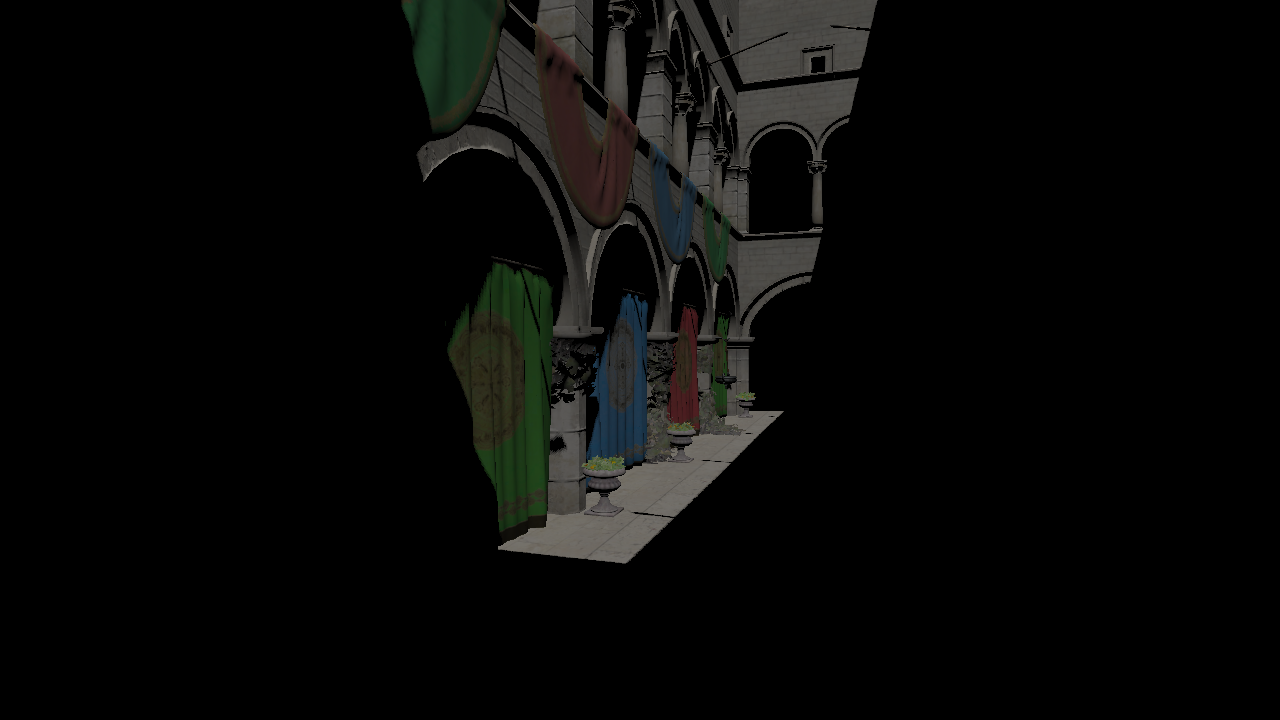
\includegraphics[width=\textwidth]{debugDirect}
%     \caption*{Direct Lighting}
%   \end{figure}
% \end{frame}

{\setbeamertemplate{frame footer}{image from Christian Eckhardt}
\begin{frame}{Indirect Lighting---Voxel Cone Tracing}
  % \begin{columns}
  %   \begin{column}{0.5\textwidth}
      \begin{block}{Voxel Cone Tracing}
        \begin{enumerate}
          \item Sample light and occlusion from the radiance texture along a particular direction
          \item Adjust level of detail as we get farther from sample point
        \end{enumerate}
      \end{block}
    % \end{column}
    % In other words, voxel cone tracing is really just raymarching but we change the level of detail as we go

    % \begin{column}{0.5\textwidth}
      \begin{figure}
        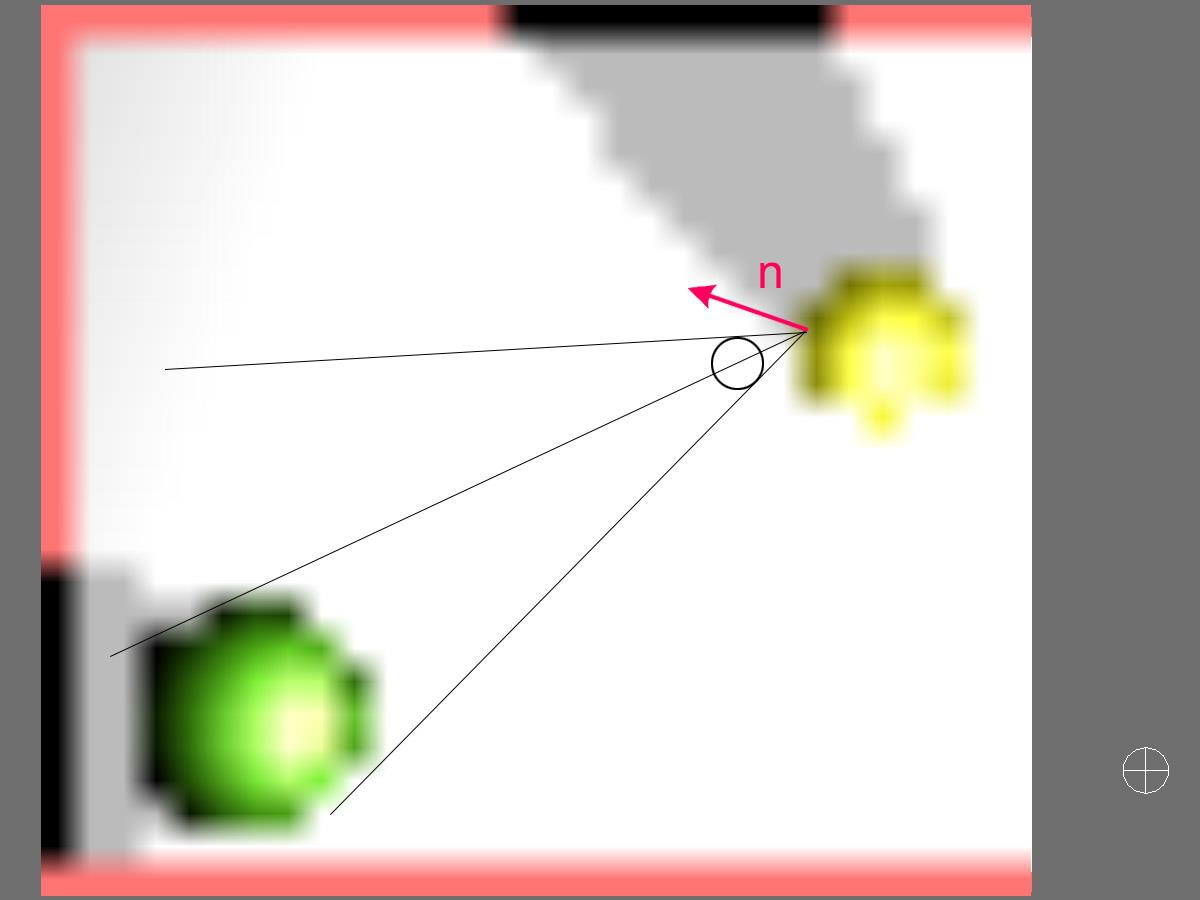
\includegraphics[height=0.5\textheight]{conetrace2}
      \end{figure}
  %   \end{column}
  % \end{columns}
\end{frame}}



{\setbeamertemplate{frame footer}{image from Christian Eckhardt}
\begin{frame}{Indirect Lighting---Voxel Cone Tracing}
% explain voxel cone tracing
% the idea (raymarching + mipmaps), choosing cone angles + dirs, diffuse indirect, specular indirect, cone tracing itself

% picture of cones again first?

% To approximate indirect lighting (recall that we are approximating a hemispherical surface integral) we use voxel cone tracing. The idea combines raytracing and mipmapping: we are raymarching through our filtered radiance values. The level to sample from is determined by the cone's diameter: at each step we increase the cone's height (also increasing the diameter)

% Here we are determining the indirect light at the point on this yellow sphere here with surface normal n. At each step, we sample from a higher level corresponding to the cone's diameter. We also are keeping track of any occlusion information and use that to blend the sampled colors together. The cone tracing stops when either the cone is fully occluded or we reach a specified number of steps.

% We use 5 cones to gather diffuse (low frequency) light and 1 cone for specular lights. The cone tracing also gives us occlusion information, which we use to attenuate the lighting.
  \begin{figure}
    \includegraphics<+>[width=0.9\textwidth]{conetrace1}
    \includegraphics<+>[width=0.9\textwidth]{conetrace2}
    \includegraphics<+>[width=0.9\textwidth]{conetrace3}
    \includegraphics<+>[width=0.9\textwidth]{conetrace4}
    \includegraphics<+>[width=0.9\textwidth]{conetrace5}
  \end{figure}
\end{frame}}

{\setbeamertemplate{frame footer}{image from \href{http://on-demand.gputechconf.com/gtc/2014/presentations/S4552-rt-voxel-based-global-illumination-gpus.pdf}{Practical Real-time Voxel-based Global Illumination for Current GPUs} by Alexey Panteleev}
\begin{frame}{Indirect Lighting---Voxel Cone Tracing}
  \begin{figure}
    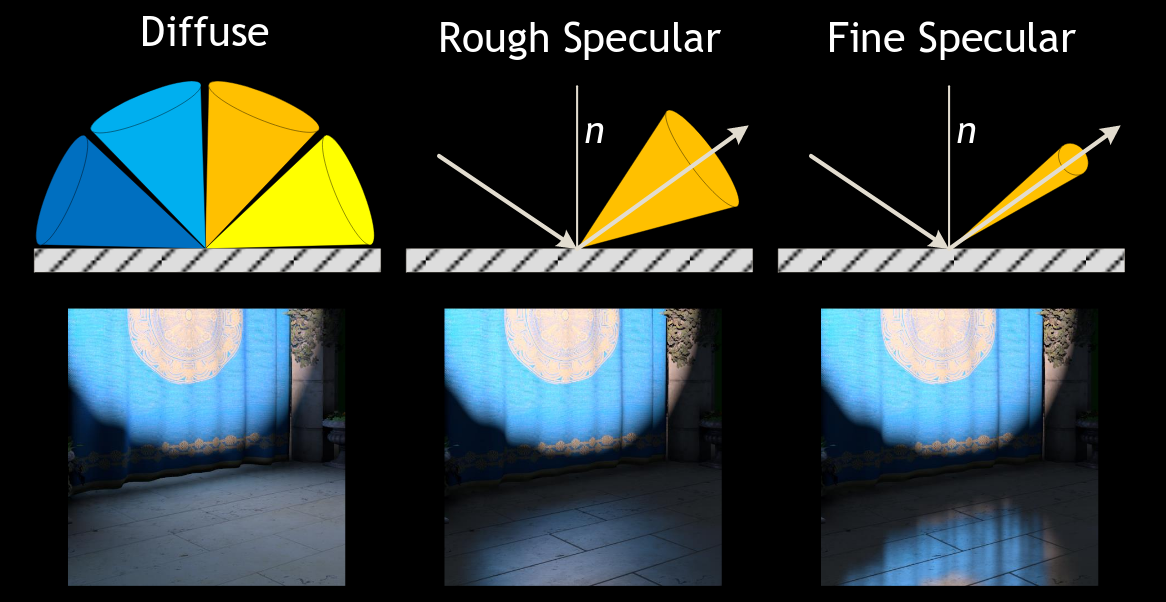
\includegraphics[width=\textwidth]{coneangles}
  \end{figure}
\end{frame}}

\begin{frame}{Indirect Lighting}
  \begin{figure}
    \includegraphics<1>[width=\textwidth]{debugIndirect_noOcclusion}
    \includegraphics<2>[width=\textwidth]{debugReflections}
    \includegraphics<3>[width=\textwidth]{debugOcclusion}
    % TODO combined total indirect lighting
    \caption*{
      \only<1>{Diffuse Indirect (no occlusion)}
      \only<2>{Specular Indirect (no occlusion)}
      \only<3>{\\Occlusion} % note this is voxel based ambient occlusion
    }
  \end{figure}
\end{frame}

\subsection{Voxel Warping}
\begin{frame}{Voxel Warping}
  \begin{itemize}
    \item Voxels are usually restricted to discrete sizes % either one size or multiples of 2
    \item What if the size is not restricted?
      \begin{enumerate}
        \item Vary with distance from camera
        % \item Size determined from low resolution occupancy information
        \item Vary based on perspective
      \end{enumerate}
  \end{itemize}
  % TODO picture of linear on one side and warped on other with guidelines (just do cubic) and show warp slope and voxels
\end{frame}

\begin{frame}{Vary with distance from camera}
  % \begin{enumerate}
  %   \item Find voxel position normalized to $[0, 1]$
  %   \item Apply `warping' function $w: [0, 1] \rightarrow [0, 1]$
  % \end{enumerate}

  % The camera is in the middle ($x = 0.5$)

  \begin{figure}
    % \begin{tikzpicture}[scale=0.8]
    %   \begin{axis}[
    %     xlabel = {linear position},
    %     ylabel = {warped position},
    %     title = {Voxel Warp Function},
    %     xmin = 0, ymin = 0, xmax = 1, ymax = 1,
    %   %   extra x ticks={0.5},
    %   %   extra x tick style={tick label style={anchor=south}},
    %   %   extra x tick labels={camera}
    %   ]
    %     \addplot[
    %       domain=0:1,
    %       samples=100,
    %     ]{0.25 * x + (3 - 3 * 0.25) * x * x + (2 * 0.25 - 2) * x * x * x};
    %     \draw[dashed] (axis cs:0.4, 0.0) -- (axis cs:0.4, 0.364) -- (axis cs:0.0, 0.364);
    %     \draw[dashed] (axis cs:0.6, 0.0) -- (axis cs:0.6, 0.636) -- (axis cs:0.0, 0.636);
    %   \end{axis}
    % \end{tikzpicture}

    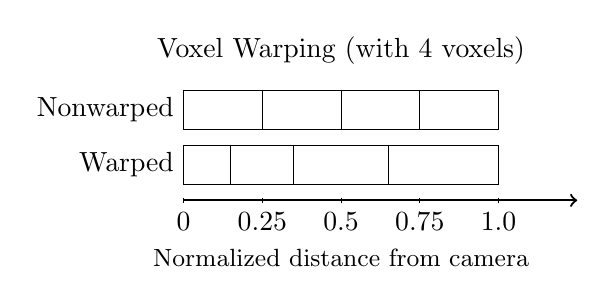
\begin{tikzpicture}
      \path (2, 1.4) node[anchor=south] {Voxel Warping (with 4 voxels)};

      \draw[black,yshift=0.7cm,xscale=4] (0, 0) rectangle (0.25, 0.5) rectangle (0.5, 0) rectangle (0.75, 0.5) rectangle (1, 0);

      \draw[black,xscale=4] (0, 0) rectangle (0.15, 0.5) rectangle (0.35, 0) rectangle (0.65, 0.5) rectangle (1, 0);

      \path[yshift=0.7cm] (0, 0.25) node[anchor=east] {Nonwarped};
      \path (0, 0.25) node[anchor=east] {Warped};

      \draw[black, ->, thick, yshift=-0.2cm] (0, 0) -- (5, 0);
      \path[yshift=-0.7cm] (2, 0) node[anchor=north,font=\small\selectfont] {Normalized distance from camera};
      \foreach \x in {0, 0.25, 0.5, 0.75, 1.0} {
        \draw[xscale=4,yshift=-0.2cm] (\x cm, 1pt) -- (\x cm, -1pt) node[anchor=north] {$\x$};
      }
    \end{tikzpicture}
  \end{figure}

\end{frame}

\begin{frame}{Vary with distance from camera}
  % \begin{figure}
  %   \includegraphics<1>[width=\textwidth]{rastervoxel_nowarp}
  %   \includegraphics<2>[width=\textwidth]{rastervoxel_warp}
  %   \caption*{\only<1>{Without warping}\only<2>{With warping}}
  % \end{figure}
  \begin{figure}
    \begin{subfigure}[t]{0.475\textwidth}
      \adjincludegraphics[width=\textwidth,trim={0 0 {0.25\width} 0},clip]{rastervoxel_nowarp}
      \caption*{Without warping}
    \end{subfigure}
    ~
    \begin{subfigure}[t]{0.475\textwidth}
      \adjincludegraphics[width=\textwidth,trim={0 0 {0.25\width} 0},clip]{rastervoxel_warp}
      \caption*{With warping}
    \end{subfigure}
  \end{figure}
\end{frame}

\begin{frame}{Vary based on perspective}
  \begin{itemize}
    \item Use perspective projection to determine voxel size
    \item Makes voxel size based on relative size in screen space
  \end{itemize}

  \begin{figure}
    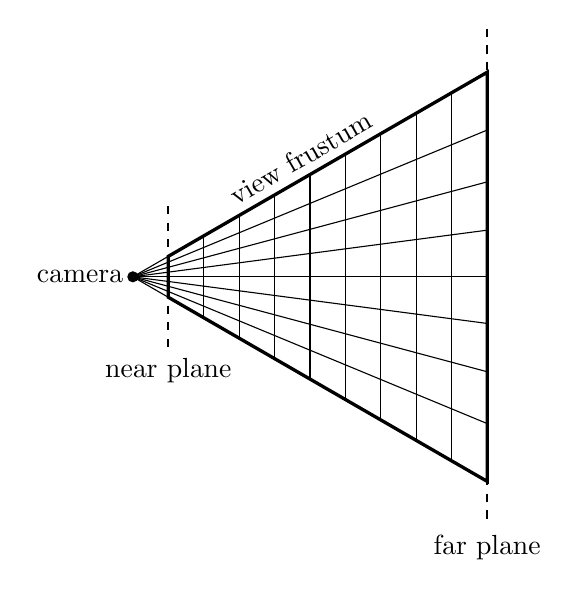
\begin{tikzpicture}[scale=0.9]
      \foreach \angle in {30, 22.5, 15, 7.5, 0, -7.5, -15, -22.5, -30} {
        \draw (0, 0) -- (5, {5 * tan(\angle)});
      }
      \foreach \z in {0.5, 1.0,...,5.0} {
        \draw (\z, {\z * tan(30)}) -- (\z, {\z * tan(-30)});
      }
      \filldraw (0,0) circle (2pt) node[anchor=east] {camera};
      \draw[dashed, thick] (0.5, 1) -- (0.5, -1) node[anchor=north] {near plane};
      \draw[dashed, thick] (5, 3.5) -- (5, -3.5) node[anchor=north] {far plane};
      \draw[very thick] (0.5, {0.5 * tan(30)}) -- (5, {5 * tan(30)}) -- (5, {-5 * tan(30)}) -- (0.5, {-0.5 * tan(30)}) -- cycle;
      \draw (2.5, {2.5 * tan(30)}) node[anchor=south, rotate=30] {view frustum};
    \end{tikzpicture}
  \end{figure}
\end{frame}

\begin{frame}{Vary based on perspective}
  % \begin{figure}
  %   \includegraphics<1>[width=\textwidth]{tessvoxels_nowarp}
  %   \includegraphics<2>[width=\textwidth]{tessvoxels_warp}
  %   \caption*{\only<1>{Without warping}\only<2>{With warping}}
  % \end{figure}
  \begin{figure}
    \begin{subfigure}[t]{0.475\textwidth}
      \adjincludegraphics[width=\textwidth,trim={0 0 {0.25\width} 0},clip]{tessvoxels_nowarp}
      \caption*{Without warping}
    \end{subfigure}
    ~
    \begin{subfigure}[t]{0.475\textwidth}
      \adjincludegraphics[width=\textwidth,trim={0 0 {0.25\width} 0},clip]{tessvoxels_warp}
      \caption*{With warping}
    \end{subfigure}
  \end{figure}
\end{frame}

\section{Results and Conclusions}

% mention somewhere that can't directly compare to other implementations so we just show our solution is viable. also need to mention the goal of voxel warping was twofold: higher resolution and, to some extent, support larger scenes (but cascaded is probably the way to go)

% \begin{frame}{Test Setup}
% \end{frame}

% First, and most important, test was to measure the general performance of the algorithm. We also varied the voxel grid resolution and screen resolution to see how it affected performance. Here are some screenshots of the varying voxel grid dimensions, starting at 64x64x64
\subsection{Results}
\begin{frame}{Results}
  % \begin{figure}
  %   \includegraphics<1>[width=\textwidth]{results_720_64}
  %   \includegraphics<2>[width=\textwidth]{results_720_128}
  %   \includegraphics<3>[width=\textwidth]{results_720_256}
  %   \caption*{
  %     \only<1>{$64^3$ voxel grid}
  %     \only<2>{$128^3$ voxel grid}
  %     \only<3>{\\$256^3$ voxel grid}
  %   }
  % \end{figure}
  \begin{figure}
    \begin{subfigure}[t]{0.475\textwidth}
      \adjincludegraphics[width=0.95\textwidth,trim={0 {0.1\height} {0.25\width} 0},clip]{results_720_64}
      \caption*{$64^3$}
    \end{subfigure}
    ~
    \begin{subfigure}[t]{0.475\textwidth}
      \adjincludegraphics[width=0.95\textwidth,trim={0 {0.1\height} {0.25\width} 0},clip]{results_720_128}
      \caption*{$128^3$}
    \end{subfigure}

    \begin{subfigure}[t]{0.475\textwidth}
      \adjincludegraphics[width=0.95\textwidth,trim={0 {0.1\height} {0.25\width} 0},clip]{results_720_256}
      \caption*{$256^3$}
    \end{subfigure}
  \end{figure}

  % analysis (which render passes were affected by what, etc)
\end{frame}

% And here we have the timing information. Each bar is for a given screen resolution and voxel grid resolution and shows the individual contributions of each render pass. For the typical 60fps goal for real-time (which is about 17ms) you see we meet the 60fps goal for all tested resolutions! I should admit this is on a GTX 970, a somewhat mid-high range graphics card, but we think these are reasonable times everything considered. I'm sure the implementation could also be optimized heavily (especially the voxelization (e.g. lower res models) and cone tracing (e.g. raymarch opts, interpolate downscaled version))
% Then talk about individual contributions (constant, varies with screen, varies with grid, with both)
\begin{frame}{Performance}
  \begin{figure}
    \pgfplotstableread[row sep=\\]{
      % Resolution Voxelize Shadowmap Inject Filter Prepass Shading\\
      % 720p64 0.90  0.69  0.92  0.04  0.20  3.89\\
      % 720p128 1.13  0.69  0.92  0.10  0.20  4.81\\
      % 720p256 2.40  0.69  0.93  0.55  0.20  5.32\\
      % 900p64 0.70  0.69  0.92  0.05  0.25  5.98\\
      % 900p128 1.12  0.69  0.92  0.10  0.26  6.42\\
      % 900p256 2.39  0.69  0.93  0.56  0.25  7.10\\
      % 1080p64 0.72  0.68  0.92  0.04  0.31  8.28\\
      % 1080p128 1.15  0.68  0.92  0.10  0.31  9.40\\
      % 1080p256 2.41  0.69  0.93  0.55  0.36  9.75\\
      Resolution Voxelize Shadowmap Inject Filter Shading\\
      720p64 0.90  0.69  0.92  0.04  4.09\\
      720p128 1.13  0.69  0.92  0.10  5.01\\
      720p256 2.40  0.69  0.93  0.55  5.52\\
      900p64 0.70  0.69  0.92  0.05  6.23\\
      900p128 1.12  0.69  0.92  0.10  6.68\\
      900p256 2.39  0.69  0.93  0.56  7.35\\
      1080p64 0.72  0.68  0.92  0.04  8.59\\
      1080p128 1.15  0.68  0.92  0.10  9.71\\
      1080p256 2.41  0.69  0.93  0.55  10.01\\
    }\dataset
    \begin{tikzpicture}[scale=0.9]
      \begin{axis}[nodes near coords ybar stacked configuration/.style={},ybar stacked, symbolic x coords={720p64, 720p128, 720p256, 900p64, 900p128, 900p256, 1080p64, 1080p128, 1080p256}, xtick=data, xticklabel style={rotate=45}, legend style={at={(1.05,0.5)}, anchor=west}, xlabel={Screen Resolution x Voxel Grid Size}, ylabel={Time (ms)}, enlarge y limits={0.2, upper}, title={Frame Times}, ymin=0]
        \addplot table[meta=Resolution, y=Voxelize] \dataset;
        \addplot table[meta=Resolution, y=Shadowmap] \dataset;
        \addplot table[meta=Resolution, y=Inject] \dataset;
        \addplot table[meta=Resolution, y=Filter] \dataset;
        % \addplot table[meta=Resolution, y=Prepass] \dataset;
        \addplot[point meta=y, nodes near coords, nodes near coords align={above}, nodes near coords style={/pgf/number format/.cd, fixed zerofill, precision=1}] table[meta=Resolution, y=Shading] \dataset;

        % \legend{Voxelize, Shadowmap, Radiance Injection, Radiance Filtering, Depth Prepass, Final Shading}
        \legend{Voxelize, Shadowmap, Radiance Injection, Radiance Filtering, Final Shading}
        % TODO try to get nested xticklabel
      \end{axis}
    \end{tikzpicture}
  \end{figure}
\end{frame}

\begin{frame}{Rasterized vs. Tessellated Voxels}
  % Opacity, color, and normals are stored in voxel textures. Since multiple shader invocations can write to the same voxel we need to use atomic operations. Both an atomic max and atomic average are supported.

  % Here's the scene colored using the rasterized voxel values. You can see some of spots where conservative rasterization didn't work completely.
  % And here are the tessellated voxels. Parts of it seem higher resolution due to not having the rasterizer produce the fragments. Also the spots where conservative rasterization didn't work well aren't an issue here. The kinda unfortunate problem though are the cracks, which are caused when the tessellation level can't get high enough, which is a hardware limitation. A possible workaround for this would be to split any large triangles when initially loading the meshes. Luckily since we'll be filtering this later most of these cracks aren't too noticeable.
  % \begin{figure}
  %   \includegraphics<1>[width=\textwidth]{rastervoxel_nowarp}
  %   \includegraphics<2>[width=\textwidth]{tessvoxels_nowarp}
  %   \caption*{\only<1>{Scene colored with rasterized voxels}\only<2>{\\Scene colored with tessellated voxels}}
  % \end{figure}
  \begin{figure}
    \begin{subfigure}[t]{0.475\textwidth}
      \adjincludegraphics[width=\textwidth,trim={{0.25\width} 0},clip]{rastervoxel_nowarp}
      \caption*{Rasterized voxels}
    \end{subfigure}
    ~
    \begin{subfigure}[t]{0.475\textwidth}
      \adjincludegraphics[width=\textwidth,trim={{0.25\width} 0},clip]{tessvoxels_nowarp}
      \caption*{Tessellated voxels}
    \end{subfigure}
  \end{figure}
\end{frame}

% Next we compared the results of the two voxelization algorithms. Visually, they are practically indistiguishable.
\begin{frame}{Rasterized vs. Tessellated Voxels}
  % \begin{figure}
  %     \includegraphics<1>[width=\textwidth]{results_voxelraster}
  %     \includegraphics<2>[width=\textwidth]{results_voxeltess}
  %     \caption*{\only<1>{Rasterized voxels}\only<2>{\\Tessellated voxels}}
  % \end{figure}
  \begin{figure}
    \begin{subfigure}[t]{0.475\textwidth}
      \adjincludegraphics[width=\textwidth,trim={0 0 {0.25\width} 0},clip]{results_voxelraster}
      \caption*{Rasterized voxels}
    \end{subfigure}
    ~
    \begin{subfigure}[t]{0.475\textwidth}
      \adjincludegraphics[width=\textwidth,trim={0 0 {0.25\width} 0},clip]{results_voxeltess}
      \caption*{Tessellated voxels}
    \end{subfigure}
  \end{figure}
\end{frame}

% Performance-wise the rasterization based approach was slightly faster. We might be able to close the gap with more optimizations. One benefit of the tessellated voxelization is the transformed points are not restricted to the viewport resolution. It also had a really convenient way to debug since we could add on a geometry and fragment shader to see where the vertices were. Also, it helped out with the voxel warping since we didn't have to worry about the viewport resolution (which controls the granularity of the fragment positions).
\begin{frame}{Rasterized vs. Tessellated Voxels}
  \begin{figure}
    \pgfplotstableread[row sep=\\]{
      Resolution Rasterized Tessellated\\
      64         0.53       0.70\\
      128        0.85       1.12\\
      256        1.91       2.35\\
    }\dataset
    \begin{tikzpicture}[scale=0.9]
      \begin{axis}[ybar=5pt, symbolic x coords={64,128,256}, xtick=data, legend style={at={(1.05,0.5)}, anchor=west}, xlabel={Voxel Grid Size}, ylabel={Time (ms)}, enlarge y limits={0.2, upper}, enlarge x limits={0.2}, title={Voxelization Time},nodes near coords, nodes near coords align={above}, nodes near coords style={/pgf/number format/fixed}, ymin=0]
        \addplot table[meta=Resolution, y=Rasterized] \dataset;
        \addplot table[meta=Resolution, y=Tessellated] \dataset;

        \legend{Rasterized, Tessellated}
      \end{axis}
    \end{tikzpicture}
  \end{figure}
\end{frame}

\begin{frame}{Rasterized vs. Tessellated Voxels}
  \begin{block}{Summary}
    \begin{description}
      \item[Rasterized:] limited by rasterizer, slightly faster
      \item[Tessellated:] limited by hardware, easier to implement
    \end{description}
  \end{block}
\end{frame}

% Lastly we evaluated our voxel warping...
\begin{frame}{Voxel Warping}
  % \begin{figure}
  %   \includegraphics<1>[width=\textwidth]{voxelwarp_off}
  %   \includegraphics<2>[width=\textwidth]{voxelwarp_on}
  %   \caption*{
  %     \only<1>{Without voxel warping}
  %     \only<2>{\\With voxel warping}
  %   }
  % \end{figure}
  \begin{figure}
    \begin{subfigure}[t]{0.475\textwidth}
      \adjincludegraphics[width=\textwidth,trim={{0.25\width} 0 0 0},clip]{voxelwarp_off}
      \caption*{Without voxel warping}
    \end{subfigure}
    ~
    \begin{subfigure}[t]{0.475\textwidth}
      \adjincludegraphics[width=\textwidth,trim={{0.25\width} 0 0 0},clip]{voxelwarp_on}
      \caption*{With voxel warping}
    \end{subfigure}
  \end{figure}
\end{frame}

\begin{frame}{Perspective Voxel Warping}
  % \begin{figure}
  %   \includegraphics<1>[width=\textwidth]{tesswarp_off}
  %   \includegraphics<2>[width=\textwidth]{tesswarp_on}
  %   \caption*{
  %     \only<1>{Without voxel warping}
  %     \only<2>{\\With voxel warping}
  %   }
  % \end{figure}
  \begin{figure}
    \begin{subfigure}[t]{0.475\textwidth}
      \adjincludegraphics[width=\textwidth,trim={{0.25\width} 0 0 0},clip]{tesswarp_off}
      \caption*{Without voxel warping}
    \end{subfigure}
    ~
    \begin{subfigure}[t]{0.475\textwidth}
      \adjincludegraphics[width=\textwidth,trim={{0.25\width} 0 0 0},clip]{tesswarp_on}
      \caption*{With voxel warping}
    \end{subfigure}
  \end{figure}
\end{frame}

\begin{frame}{Voxel Warping}
  \begin{itemize}
    \item Adaptively change voxel resolution
    \item Bad artifacts when objects move (looking into ways to fix this) % when the voxel sizes are discrete we can snap the voxel grid to eliminate flickering. If the voxel sizes are continuous we can't do this. We tried a couple things like temporal filtering to make this better but it still isn't great. (part of future work)
  \end{itemize}
\end{frame}

% \newcommand{\smallcolumns}[4][0.5, 0.5]{\begin{columns}\begin{column}{#1\textwidth}#3\end{column}\begin{column}{#2\textwidth}#4\end{column}\end{columns}}
\subsection{Related Work}
\begin{frame}{Related Work}
  How does it compare with other methods?
  \vspace{1cm}

  % From the beginning I mentioned some general steps most gi algorithms follow. I'd like to point out how our work compares to some other related work by quickly going through each of these points with a few other techniques as presented in their research papers.
  Important parts of global illumination algorithms:
  \begin{enumerate}
    \item Scene representation? % what information do we use for the lighting?
    \item Light computation? % how is the lighting computed? is there any intermediate computation required before the final light sampling?
    \item Light sampling? % how do we sample the lighting?
  \end{enumerate}
\end{frame}

% {\setbeamertemplate{frame footer}{image from \href{https://dl.acm.org/citation.cfm?id=1053460}{Reflective shadow maps} by C.\ Dachsbacher and M.\ Stamminger}
% \begin{frame}{Related Work---Reflective Shadowmaps}
%   \begin{enumerate}
%     \item Scene representation? \alert{Reflective shadowmap (RSM)}% reused from shadowmap
%     \item Light computation? \alert{None, use color and normal from RSM}% normal and color stored along with shadowmap
%     \item Light sampling? \alert{Sample nearby points in RSM} % project point into the RSM and sample nearby points
%   \end{enumerate}

%   \begin{figure}
%     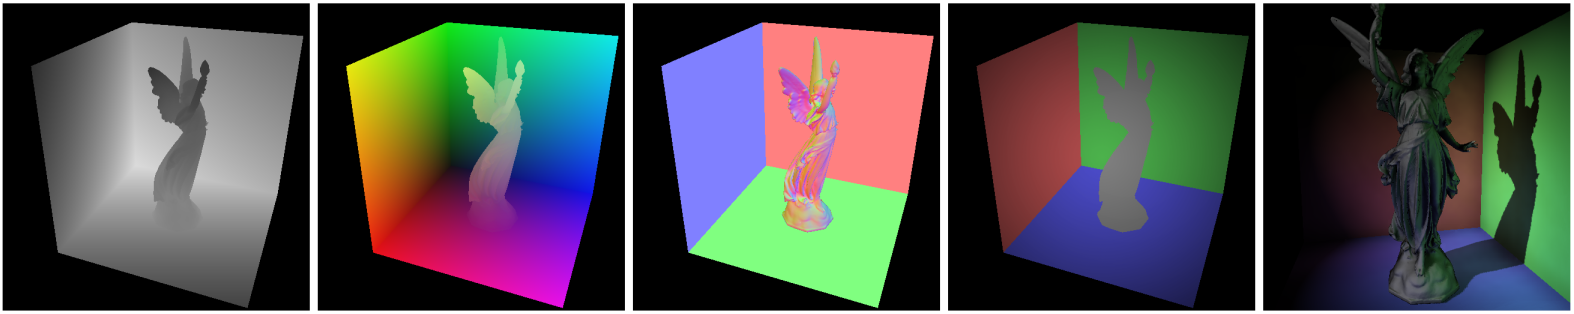
\includegraphics[width=\textwidth]{rsm}
%   \end{figure}

%   % pros straighforward, doesn't require any fancy data structures
%   % cons no occlusion information and complexity linear wrt number of lights, no specular
% \end{frame}}

{\setbeamertemplate{frame footer}{image from \href{http://www.crytek.com/download/Light_Propagation_Volumes.pdf}{Light Propagation Volumes in CryEngine 3} by A.\ Kaplanyan}
\begin{frame}{Related Work---Light Propagation Volumes}
  \begin{enumerate}
    \item Scene representation? \alert{Voxel grid (incomplete)}% low resolution voxel grid (originally this wasn't a complete voxelization---it was constructed from other info like shadowmap and depth information), stored in (cascaded) 3d texture
    \item Light computation? \alert{Iterative propagation} % light is iteratively propagated/filtered to neighboring voxels until the information is stable
    \item Light sampling? \alert{Texture lookup} % simple lookup into voxel texture
  \end{enumerate}

  \begin{figure}
    \centering
    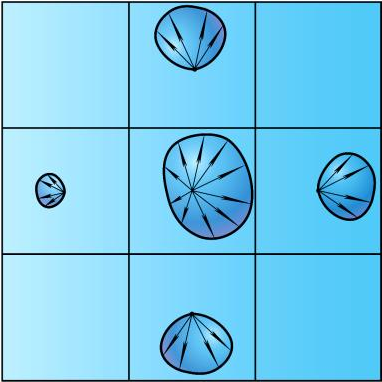
\includegraphics[height=0.5\textheight]{lpvpropagation}
  \end{figure}


  % pros stable lighting, smaller memory requirements since lower resolution grid
  % cons occlusion info not complete, no specular
\end{frame}}

{\setbeamertemplate{frame footer}{image from \href{http://research.nvidia.com/sites/default/files/pubs/2011-09_Interactive-Indirect-Illumination/GIVoxels-pg2011-authors.pdf}{Interactive Indirect Illumination Using Voxel Cone Tracing} by C.\ Crassin et al.}
\begin{frame}{Related Work---Voxel Cone Tracing}
  \begin{enumerate}
    \item Scene representation? \alert{Sparse voxel octree}% high resolution voxel grid (in sparse voxel octree, in vxgi in clipmap). also this is where the rasterized voxelization approach came from
    \item Light computation? \alert{Mipmaps} % make mipmaps, the same as our implementation
    \item Light sampling? \alert{Voxel cone tracing} % voxel cone tracing
  \end{enumerate}

  \begin{figure}
    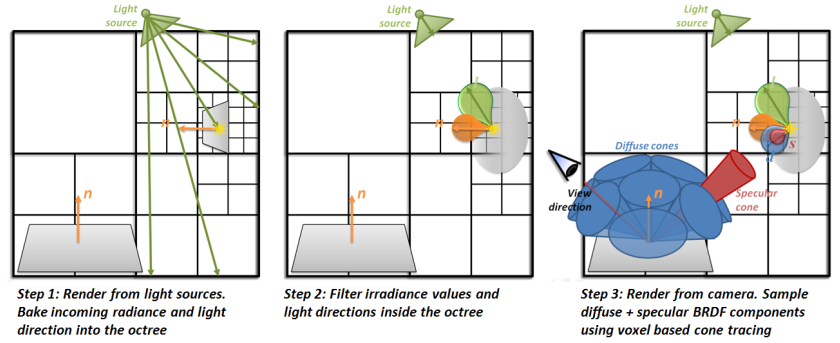
\includegraphics[width=\textwidth]{vct}
  \end{figure}


  % pros specular
  % cons octree is complicated (especially if scene is dynamic since octree nodes need to be managed well), clipmap also somewhat complex and still uses lots of memory
\end{frame}}

% \begin{frame}{Related Work---Ours}
%   \begin{enumerate}
%     \item Scene representation? \alert{Warped voxel grid} % high resolution voxel grid (in warped 3D texture). tessellated voxelization (side note: we briefly checked if this had been done already and didn't find anything at first. after implementing it we looked again and found a single paper on ACM from 2012 with a citation count of 0 and 252 cumulative downloads ever)
%     \item Light computation? \alert{Mipmaps} % make mipmaps
%     \item Light sampling? \alert{Voxel cone tracing} % voxel cone tracing
%   \end{enumerate}

%   % So what we really gained from looking into the voxelization is that warped voxels might be viable if the temporal issues can be fixed. The tessellated voxelization might help with that since we can work with the arbitrary vertex coordinates instead of having to effectively truncate them to rasterized fragments (we don't lose precision)

%   % pros simple, has specular, adaptive resolution
%   % cons warping suffers from flickering
% \end{frame}

% TODO related works summary slide? pros/cons on each related work slide?

\subsection{Conclusion}
\begin{frame}{Conclusion}
  % wrap up and list contributions again
  \begin{itemize}
    \item Implementation\footnote{Find the source here: \url{github.com/sfreed141/vct}} of real-time global illumination using voxel cone tracing
    \item Implementation and comparison of two voxelization methods
    \item Investigation into warped voxels
  \end{itemize}
\end{frame}

\begin{frame}{Future Work}
  % other ways of adjusting resolution are more feasible due to temporal artifacts

  % Follow ups for voxelization and voxel warping, then general improvements

  \begin{itemize}
    \item Try to alleviate flickering with warped voxels % temporal, hole filling, voxel interpolation, snapping % not restricted by rasterizer so we can put vertices where we want % voxels corresponding to view frustum still interesting idea, finding a way to reduce flickering would be great
    \item Fully implement LPVs and VCT (as described in research paper) for direct comparison % can't really do this right now since there are too many differences between engines to make a fair comparison. also what assets do they use and what other techniques?
    \item Cascaded sparse 3D textures % uniform voxels (clearly) easier to work with. sparse textures might help alleviate memory consumption issues without having to resort to an octree
    % \item Solid voxelization % as opposed to surface voxelization like now. rasterization vs tessellation doesn't matter much (even with optimizations most likely)
    \item Spherical harmonics, anisotropic filtering, adaptive cone tracing quality, other miscellaneous optimizations % staggered updating of filtered radiance, voxelizing with lower level of detail mesh, cone trace at lower resolution and interpolate
  \end{itemize}
\end{frame}

\begin{frame}[standout]
  \LARGE Thank you!\\
  \vspace{1cm}
  \LARGE Questions?
\end{frame}

% TODO bibliography slides?

\end{document}
